\documentclass[11pt,a4paper]{report}
\usepackage[utf8]{inputenc}
\usepackage[T1]{fontenc}
\usepackage{amsmath}
\usepackage{amsfonts}
\usepackage{amssymb}
\usepackage{graphicx}
\usepackage{xcolor}
\usepackage{caption}
\usepackage{subcaption}

\usepackage{biblatex}
\bibliography{database} % or
% \addbibresource{<database>.<extension>}

%// DON'T FORGET TO RUN BIBER ON database.bib !!!

\usepackage{listingsutf8}
\usepackage[cache=false]{minted}

\usepackage{algorithm}
\usepackage{algpseudocode}

\usepackage{array}

% Note: these commands allow to write "commits" easily and in a readable manner. For final delivery, all you need it to remove the internals of the macro, so that all "commits" will be replaced by blanks.
\definecolor{Brown}{rgb}{0.4,0.1,0.2}
\definecolor{Red}{rgb}{1,0,0}
\definecolor{Green}{rgb}{0,1,0}

\newcommand{\commitalt}[3]{\begin{minipage}{\textwidth}\bfseries\colorbox{Red}{\textcolor{white}{#1}}\colorbox{blue}{\textcolor{white}{#2}}\newline\parbox{0.45\textwidth}{\colorbox{Red}{\textcolor{white}{#3}}}\end{minipage}}

\newcommand{\commit}[3]{\begin{minipage}{\textwidth}\bfseries\colorbox{Green}{\textcolor{black}{#1}}\colorbox{blue}{\textcolor{white}{#2}}\newline\parbox{0.45\textwidth}{\colorbox{Green}{\textcolor{black}{#3}}}\end{minipage}}

\newcommand{\commitread}[3]{\begin{minipage}{\textwidth}\bfseries\colorbox{Brown}{\textcolor{white}{#1}}\colorbox{blue}{\textcolor{white}{#2}}\newline\parbox{0.45\textwidth}{\colorbox{Brown}{\textcolor{white}{#3}}}\end{minipage}}


\newcommand{\warn}[1]{{\huge \color{red} \bfseries {#1} }}

\newcolumntype{L}[1]{>{\raggedright\let\newline\\\arraybackslash\hspace{0pt}}m{#1}}
\newcolumntype{C}[1]{>{\centering\let\newline\\\arraybackslash\hspace{0pt}}m{#1}}
\newcolumntype{R}[1]{>{\raggedleft\let\newline\\\arraybackslash\hspace{0pt}}m{#1}}

%\newcolumntype{C}[1]{>{\centering\arraybackslash}m{#1}}
%\newcolumntype{L}[1]{>{\raggedleft\arraybackslash}m{#1}}
%\newcolumntype{R}[1]{>{\raggedright\arraybackslash}m{#1}}

\author{Jonathan LEVY}
\title{Master thesis \\ Acceleration of Seed Extension for BWA-MEM DNA Alignment Using GPUs}
\begin{document}
	\maketitle
	
	\section*{Abstract}
	\begin{abstract}
.DNA aligning is a compute-intensive and time-consuming task required for all further DNA processing. It consists in finding for each DNA string from a sample its location in a reference genome. Usual techniques for short reads (hundreds of bases) involve seed-extension, where a small matching seed is found with quick search through FM-index, and then extended on both ends with a custom Smith-Waterman algorithm, giving optimal solution. However, this seed-extension takes a tremendous amount of time. This is why we present in this thesis a solution to offload extension on a GPU to be done in a parallel fashion. This is possible thanks to the fact that the DNA reads do not present any kind of relation between each other. We used the Burrows-Wheeler Aligner (BWA), a reference program in the field, to which we integrated a GPU-accelerated library for extension, GASAL2. However, BWA has a left-right dependency on extension starting scores, with the left alignment starting with the seed score, then the right part starting with the previously calculated left score. We designed a solution by starting both extensions with the seed score, we called this method the "seed-only" paradigm. On our test machine featuring 12 hyperthreaded cores and an NVIDIA Tesla K40c, when running with 12 threads, we could observe a raw kernel speed-up of 4.8$\times$ ; but if we allow non-blocking calls to let the CPU run the seeding tasks while the GPU computes the extension, we can reach a 16$\times$ effective speed-up. This extension part takes around 27\% of the total time but our acceleration introduces a small overhead due to memory preparations and copying, which makes the whole application 1.28$\times$ faster, getting close to the theoretical maximum of 1.37$\times$. Additionally, the paradigm shift we operated creates a negligible difference in the final overall scores, with a 0.23\% difference for our 5.2 million sequences data set. This makes our acceleration with GASAL2 an efficient solution for a single machine that preserves results.
\end{abstract}

	
	\tableofcontents
	
	\chapter{Introduction}
	\label{chap:intro}
	The work in this thesis is about using the latest computing techniques available to speed up a bioinformatics application. To understand the context in which this work takes place, an introduction to some biological concepts is presented in this chapter.
	
		\section{Context}
		
DNA is the general medium of information common to all known living creatures. It defines all the traits that all the individuals from a species share, and thus, is the most important source of biological information for species definition and the understanding of life in general. This code is replicated when a cell goes under mitosis, ensuring that the whole organism has a coherent DNA code across all its cells.

DNA takes the form of a long string of proteins, linked two by two. These proteins are called "nucleotides" or "bases", as they are the base of the DNA code. There are four of them: adenine [A], thymine [T], cytosine [C] and guanine [G], often referred to by their initial for ease of use. Adenine and thymine are linked together, and cytosine and guanine are also paired together, forming a double-helix, as shown on Figure~\ref{fig:double-stranded-dnamed}.

\begin{figure}[h]
	\centering
	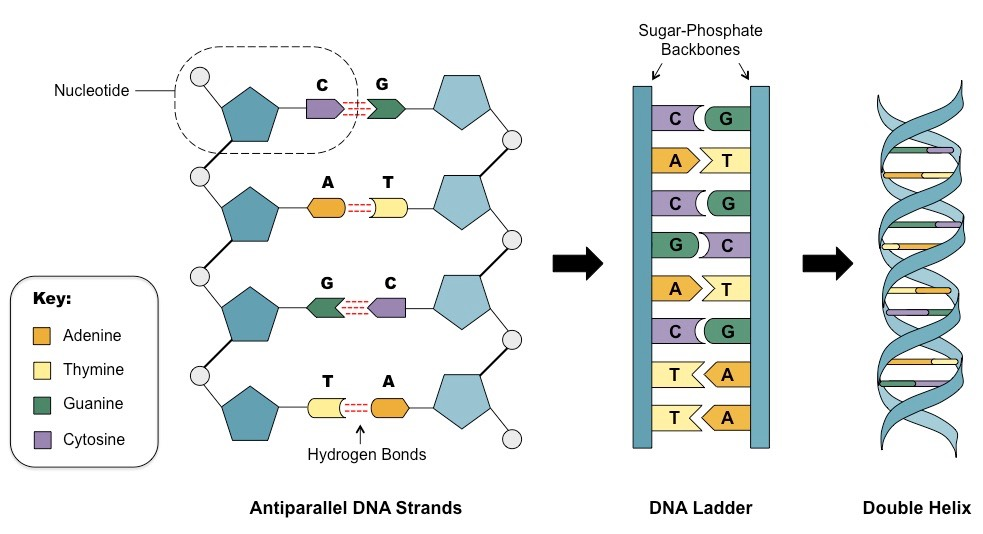
\includegraphics[width=1\linewidth]{double-stranded-dna_med}
	\caption{DNA double-helix with nucleotides (from~\cite{cornell:dnastructure})}
	\label{fig:double-stranded-dnamed}
\end{figure}


An important factor of differentiation in the characteristics in different species is mutation, when a random modification appears in the DNA code and propagates across the population with reproduction. If the mutation gives the bearer an advantage in life over the non-bearers, it has a high probability to get passed to the bearer's descendants, fostering its propagation in the population (for example, having coloured petals for flowers makes them attractive for insects, and since coloured flowers have become more pollinated, their heirs will inherit this trait). On the contrary, if the mutation becomes a drawback, it is unlikely to be passed to the descendants.

Some genetic mutations are proven deadly, and the most well-known in this category is cancer. A cell whose DNA has been damaged or altered can start multiplying in an uncontrollable fashion, creating a pack of cells growing ever bigger, becoming malign and threatening the normal behaviour of an organ. This process, known as carcinoma, can be detected by multiple ways, some more empirical than others (for example, an easy setup with X-rays can allow a doctor to detect a small abnormal spot, which could be a sign of carcinoma). One way to detect this is by getting a sample of DNA from a patient, and comparing it with a known reference.

To achieve this comparison, one needs to find which area of the reference genome matches with the samples, or said differently, one needs to align the sample DNA with the reference and find how similar these two are. Consequently, we define a metric to quantify that closeness, called the \emph{alignment score}.

In this case, only a pair of sequences are being matched: a sample, and a reference. This is called \emph{pairwise alignment}. Other cases where DNA alignment is needed can involve comparing multiple species' DNA to find regions that share some similarity, and that could translate into shared trait among species. In that situation, multiple sequences are mapped together, which makes it yet another problem.
		
		\section{DNA alignment, a time-consuming process}
		Mapping is the process of finding the location in the reference genome where a DNA read from a sample probably belongs to. Since 99\% of the genome is the same in a species, finding the location in the reference genome is similar to identify the position of a read in the sample DNA. Moreover, the mapping must also provide the information about how well the read is aligned to the reference genome giving the exact location and nature of each kind of mutation (insertion, deletion or modification of one or multiple bases).  Mapping DNA reads is a complex task due to large sequencing data and reference genome size. Different types of mutations also increase the complexity of the mapping. In the case of the human, we can write the whole sequence of nucleotides with A, T, C, and G letters, just like a long string of characters. If each character is encoded on a byte, the whole text would be around 3.4GB. Even though it seems small regarding today's standards of data storage, looking for a particular area that would match a string is far from trivial. As such, a sophisticated way to look into the genome and find an alignment is needed.


At the moment, DNA mapping represents the first genomics analysis step of many DNA analysis approaches in practice. The complicated process of DNA mapping is rather time consuming, both due to the high complexity of the analysis involved as well as the amount of data that needs to be processed. In many cases, mapping can take between $30\%$ and $50\%$ of the total DNA analysis time. Figure~\ref{fig:pipelineprocesstime} shows that the time taken by mapping which is about a third of the total pipeline time. Moreover, the time taken for this part is counted in thousands of CPU-core hours for this example data set. Therefore DNA mapping is a computational challenge and various techniques to achieve it in a timely manner. The problem at stake is then to find an effective way to compute DNA alignment as fast as possible.

\begin{figure}[h]
	\centering
	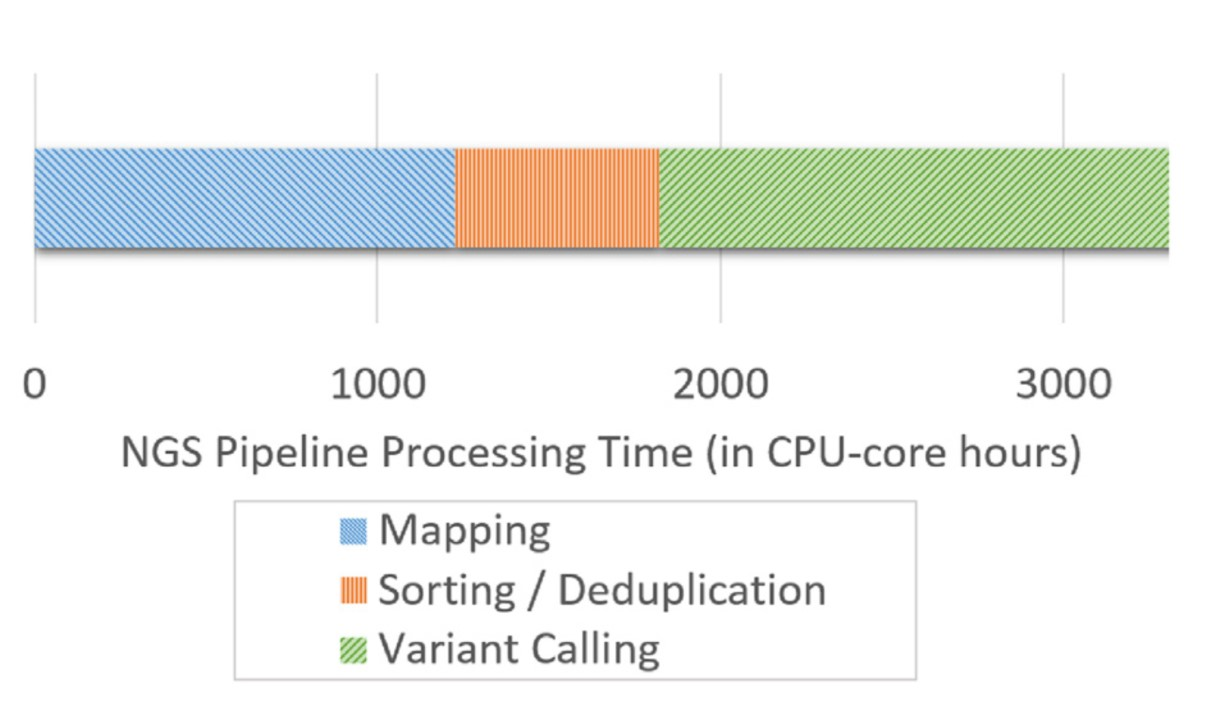
\includegraphics[width=1\linewidth]{pipelineprocesstime}
	\caption{DNA pipeline process time share for a typical 30$\times$ coverage cancer DNA data set. The data set consists of three tumor samples and one normal tissue sample (time given in CPU-core hours). (from~\cite{HOUTGAST201854})}
	\label{fig:pipelineprocesstime}
\end{figure}


% refer to that paper : https://www.sciencedirect.com/science/article/pii/S1476927118301555 and also show the figure in the paper (copy it and use a reference)

		
		\section{The alignment problem}
		%% Introduce what sequencing machines are in the context
Several questions arise from the problem of computing DNA alignment. First, we introduced the fact that the alignment should provide some kind of metric, to quantify how good the alignment is. A sample DNA is constituted of a large number of strings, all of them having the same number of bases (for example, 150 bases). This is because sequencing machines output fixed-length strings. These fixed-length strings are called \emph{query} sequences. Each of them should be aligned with a slightly longer sequence located in the reference genome. All of these sequences extracted from the genome are called the \emph{target} sequences.

As said before, these two sequences are composed of nucleotides or bases, which are reported from their first letter: A, T, C and G. We define a match score corresponding to the score when two bases are equal. In the case of DNA, mutations often take the form of adding bases, deleting bases, or changing some bases, as seen on figure~\ref{fig:mutation}. 
\begin{figure}[h!]
	\centering
	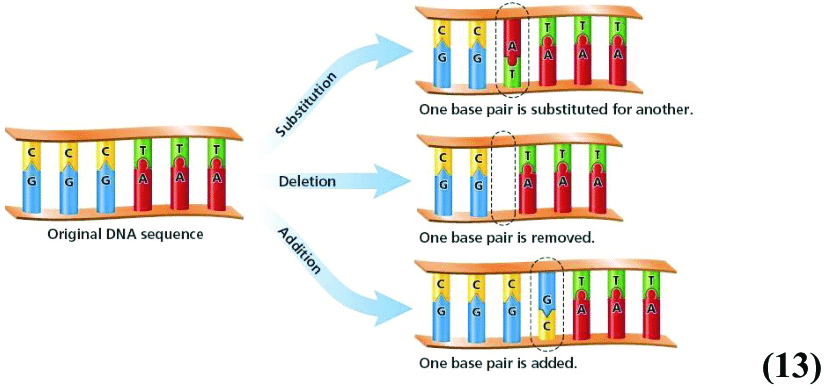
\includegraphics[width=1\linewidth]{mutation}
	\caption{Examples of mutation (from~\cite{alasadi:chemistry})}
	\label{fig:mutation}
\end{figure}
Mismatches can appear in the form of insertion or deletion of one or multiple bases, in either the query or the target. We then define an insertion mismatch score and a deletion mismatch score. The matching score has a positive value, and the mismatch scores are negative, and often mismatch scores are set at the same value. For the query sequences, it may happen that a base cannot be correctly retrieved by the sequencing machine, and if this happens, the unknown base is denoted as "N" and is always counted as a mismatch. Furthermore, in real-life mutations, it is much more likely to have a small number of long gaps rather than multiple short gaps. To reflect this, the model "affine gap penalty" for DNA mutation is used. We define a big mismatch score for opening a gap, and a smaller mismatch score for extending the gap. This way, during the alignment, we apply a bigger penalty when trying to open a gap rather than when a mismatch only causes a gap to get wider. 

Another challenge is to process a huge number of sequences as fast as possible. In fact, DNA sequencers produce DNA strings of a given length proper to each machine. While older sequencers produce short strings of 80 or 150 bases, more recent ones can output 7000 bases per string, and millions of strings are produced. Thanks to the fact that strings are not related to each other. There is no obstacle in processing multiple of them at the same time. This mode is called \emph{inter-sequence parallelisation}. It is also possible to parallelize the alignment calculation for each sequence, but this mode, named \emph{intra-sequence parallelisation}, requires extra care about synchronisation.

Furthermore, looking into a full genome for a match would be an incredibly tedious task without an efficient search algorithm. It is then advisable to create an index of the reference genome. With this index, operations to research a given pattern in a huge data set can be faster than linear time with respect to the data size.


	
		\section{Thesis overview}
		This thesis is organised as follows. 
In Chapter~\ref{chap:background}, an overview of the background to understand DNA alignment is given. We also provide explanations about GPU computing and its usage in this application. This aims to show the reason why we chose this approach to solve the problem of DNA alignment.

Chapter~\ref{chap:accel} contains details about the accelerator discussed in this thesis. While it originally supported few features, more functionality and flexibility are added and its integration to an existing aligning software is presented.

The implementation of proposed improvements is shown in Chapter~\ref{chap:implementation}. In particular, we provide a detailed view of how we adapted the original software to include our accelerator. We also review the modifications we brought to our solution to integrate it successfully.

Chapter~\ref{chap:measurements} presents the experimental setup used to test the implemented accelerator and also discusses the measurement results showing its performance and accuracy.

Finally we will conclude in Chapter~\ref{chap:ccl} with the final thoughts and possible future works.
		
	\chapter{Background}
	\label{chap:background}
		\section{DNA alignment}
		DNA alignment comes at a time where sequencing machines become more and more available and affordable. The principle behind alignment is to find a match between \emph{reads} coming out of a sequencing machine in a given \emph{reference} genome. 

To achieve this in a timely manner, most software rely on the \emph{seed-and-extend} technique.

In the first step, the \emph{seeding} part consists in finding a substring of a given length that matches exactly in the read and in the reference. Depending on the parameter used in various software, a maximum of zero, one, or several mismatches can be allowed. For this step, it is necessary to look into the whole genome for a match, and an index is used. One indexing algorithm relies on the Burrows-Wheeler transform~\cite{BurrowsWheeler:align}, and is used in many DNA aligners today. During this step, multiple seeds can be found in various parts of the reference genome, and depending on how they overlap, they can be grouped in chains. Then for all chains, an extension is performed.

The extension part consists in trying to pursue the alignment started from the chain on both sides, left and right. If the chain is located at the beginning or the end of the sequence, only one alignment is needed. More refinements are possible, for example, detecting if the score is dropping when continuing the alignment, and cutting the calculation to avoid computing useless parts; or only computing probable aligning positions, and skipping the highly unlikely ones. %These algorithms will be detailed in the next section.


		
		\section{Seed-extension}
		In this section, we will detail the algorithms discussed earlier.

First, let's review the seeding algorithm. We will quickly introduce the benefits of using the Burrows-Wheeler transform to build an index. This transformation is used in the FM-index.

The FM-index is a compressed representation for the reference genome. It is widely used thanks to its lightweight memory footprint, which is sub-linear with respect to the size of the data. Searching for a pattern in the compressed text is also sub-linear in time, which makes it ideal for seeding. When a seed is located, a chunk is taken from the genome around the seed to perform the alignment with the query sequence. This chunk should be larger than the query with which it shares a seed, since there could be gaps in the alignment. More details are available online~\cite{wiki:FMIndex}, but the following work does not rely on how FM-index works. 
%% You could detail the algorithm more, but who cares.

After seeding, we have to continue to align on both sides of the chain. For the extension, dynamic programming algorithms are used. They may be compute-intensive (and compute-bound), but they provide an optimal solution to the alignment problem. We could actually use them to compute the whole alignment but it is much more efficient to run smaller alignments as left and right extensions of the seed. They rely on computing a matrix of size $N \times M$, $N$ and $M$ being the length of the query and target sequences respectively. As shown on Figure~\ref{fig:dpmatrix}, we place the target sequence as a row, and the query as a column. Each cell is filled with a score depending on the north cell, the west cell, and the north-west cell, and the current bases to align. For the pair of bases, it corresponds to row and the column. For the sake of simplicity, let's assume that we only count matches with a score $\alpha > 0$, mismatches with a score $\beta < 0$, and a score for insertion and deletion $\gamma < 0$. We define the relation for the score $S_{i,j}$ on cell $i,j$ related to bases $a_i$ and $b_j$ with the formula~\ref{equ:dp}. In the Figure~\ref{fig:dpmatrix}, $\alpha = 2$ and $\beta = \gamma = -1$. More detailed information can be found in ~\cite{Aluru:2005:HCM:1121650}.

\begin{equation}
	S_{i,j} = max \left\{
	\begin{array}{llll}
		S_{i-1, j-1} + \alpha & \mbox{if} & a_i = b_j \\
		S_{i-1, j-1} + \beta & \mbox{if} & a_i \neq b_j \\
		S_{i, j-1} + \gamma \\
		S_{i-1, j} + \gamma\\
		 \\
	\end{array}
	\right.
	\label{equ:dp}
\end{equation}



\begin{figure}[ht!]
	\centering
	\begin{subfigure}[t]{0.5\textwidth}
		\centering
		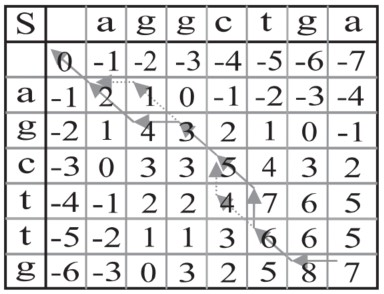
\includegraphics[height=0.5\textwidth]{global_align}
		\caption{Global alignment}
		\label{fig:global_align}
	\end{subfigure}%
	~ 
	\begin{subfigure}[t]{0.5\textwidth}
		\centering
		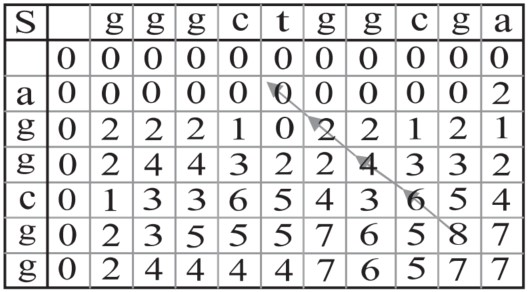
\includegraphics[height=0.5\textwidth]{local_align}
		\caption{Local alignment}
		\label{fig:local_align}
	\end{subfigure}
	\caption{Dyanmic programming alignments (from ~\cite{Aluru:2005:HCM:1121650}) }
	\label{fig:dpmatrix}
\end{figure}



Among dynamic programming (DP) algorithms, we can cite main techniques:

\begin{itemize}
	\item Needleman-Wunsch~\cite{NeedlemanWunsch:method}, or \emph{global} alignment: it tries to match the whole sequences. The results contains both sequences completely, as Figure~\ref{fig:global_align} shows, with the alignment path traversing the matrix. Mismatches on ends causes a penalty, as shows the negative scores on the edges;
	\item Smith-Waterman~\cite{SmithWaterman:identification}, or \emph{local} alignment: it aligns two sequences but only looks for the maximal score, which reports the best alignment there is. On Figure~\ref{fig:local_align}, one can see we select the best score, the score is initialised at 0 and stays positive;
	\item A mix of the two, \emph{semi-global}~\cite{Durand:course-genomics} alignment, that performs a global alignment but allows to skip both ends of the query sequence. In practical, semi-global is often used instead of global;
	\item BLAST~\cite{Altschul:BLAST}-like extension: it performs two alignments on both ends of the seed instead of aligning the sequences entirely. If first makes a local alignment on the left side, starting with a non-zero score, but taking the seed score instead. Then it makes a local alignment on the right side, starting as initial score the previous computed score (taking the seed and left alignment). This splits the alignment problem in two, which makes it much faster. This is the technique used in seed-extension.
\end{itemize}

The pseudocode for local alignment is presented in Algorithm~\ref{algo:local}. It computes the whole dynamic programming matrix $S$ with the equation~\ref{equ:dp} showed above. There are small difference between global, local and semi-global alignments in the initialisation step, the computing formula, and how the final score is obtained from the matrix. For the local alignment, which is the one we will use in the rest of the thesis, initialisation is done with a score of zero along both north and west edges of the matrix. This means that no penalty is made on the ends of both sequences. Second, in the computing formula showed in equation~\ref{equ:dp}, the score can actually go negative if a lot of mismatches occur. We do not want this behaviour with local alignment, meaning that there is no penalty if an area is not aligned (the alignment can occur later on in the sequence). In the Algorithm~\ref{algo:local}, this is shown by taking the maximum of the computed score with 0. Finally, in local alignment, we want the best possible score without constraints on the end of the alignment, so we simply take the maximum value in the dynamic programming matrix as the end position of the alignment.

\begin{algorithm}[h!]
	\caption{Dynamic programming matrix computation algorithm}
	\label{algo:local}
	\begin{algorithmic}[1] % The number tells where the line numbering should start
		\Procedure{Compute the dynamic programming matrix, local alignment}{$query\_string$, $target\_string$, $query\_length$, $target\_length$} \Comment{}
		

		\State \emph{Initialise score}
		\For{i from -1 to $query\_length$}
			\State $S_{i, -1} \leftarrow 0$
		\EndFor	
				
		\For{j from -1 to $target\_length$}
			\State $S_{-1, j} \leftarrow 0$	
		\EndFor
		
		\State \emph{compute S matrix}
		\For{ (i from $0$ to $query\_length - 1$}
			\For {j from $0$ to $target\_length - 1$}
			
				\State Read base $query\_base_i$ in $query\_string$
				\State Read base $target\_base_j$ in $target\_string$ 	
				\State $ 	S_{i,j} \leftarrow max \left\{
				\begin{array}{llll}
				S_{i-1, j-1} + \alpha & \mbox{if} & query\_base_i = target\_base_j \\
				S_{i-1, j-1} + \beta & \mbox{if} & query\_base_i \neq target\_base_j \\
				S_{i, j-1} + \gamma \\
				S_{i-1, j} + \gamma\\
				0 \\
				\end{array}
				\right. $
				
			\EndFor
			
		\EndFor
		
		\State Find $i_{max}$ and $j_{max}$ for which $S_{i_{max}, j_{max}} = max(S_{i,j})$
		\State $score \leftarrow S_{i_{max}, j_{max}}$
		\State $end\_position\_query \leftarrow i_{max}$
		\State $end\_position\_target \leftarrow j_{max}$
		
		\EndProcedure
		
	\end{algorithmic}
\end{algorithm}

On these algorithms, several optimisation can be added to speed them up. Depending on the technology at hand, one can use Single Instruction Multiple Data (SIMD) to compute several cells of the dynamic programming matrix at once. Another optimisation called \emph{z-dropoff} is interrupting the calculation of a row when the score drops sharply. Finally, it can be noticed that the north-east and south-west corners of the dynamic programming matrix are often useless to compute, since reaching these cells would mean that the alignment is containing a huge gap (and hence has a mediocre score). One can simply avoid to compute them, resulting in only calculating a band around the diagonal, hence calling this technique banded dynamic programming.

		
		\section{Alignment on GPU}
		DNA computation can take advantage of the inner structure of a GPU to compute the alignment faster. First, we will quickly recap the current solutions at hand. Then a presentation of the GPU architecture and programming paradigm will show how this device work and how they are adapted for this work.

\subsection{Parallel computing for DNA alignment}

The computation for alignment between two DNA strings is intensive, yet simple. The main problem comes from the input data size. Still, it is important to note that each pair of alignment is independent from the others. A simple and effective way to accelerate the computation is to parallelise it. On a computer, one can use multiple threads on a CPU to achieve that parallelisation and compute several alignments at the same time. However, the number of threads available on a CPU is limited to a dozen, or a few dozen at best; but Graphics Computing Units (GPUs) can have hundreds to thousands of cores at disposal. This makes GPUs a hardware of choice for acceleration using parallel computing. Running multiple alignments in parallel is called \emph{inter-sequence parallelistion}.

It is possible to go even further with \emph{intra-sequence parallelisation}, that is, to calculate the dynamic programming matrix with multiple threads. This implies having synchronisation phases: since the cell values depends on the previously calculated ones, it implies some sort of logic order. However, we will not explore this topic later on.

As for current solutions, a quick list of some of the existing software for DNA alignment will be presented. These tools are most often present as libraries, to be able to integrate them in bigger and more easy-to-use software.

\begin{itemize}
    \item \emph{SeqAn} is a C++ toolbox for DNA alignment. It features a lot of various tools, and implements its own C++ library for alignment. It runs on multiple CPU threads, and can rely on SIMD for moderate acceleration,
    \item \emph{Basic Local Alignment Seach Tool} (\emph{BLAST}) searches for pairwise alignment with the seed-extension method,
    \item \emph{Burrows-Wheeler Aligner} (\emph{BWA}) is a DNA aligner focused on speed relying on FM-index for seeding, with BLAST-like extension,
    \item \emph{NVBIO} is a GPU-accelerated library written in CUDA, the dedicated language for general-purpose GPU computing on NVIDIA GPUs. It has a lot of features including banded dynamic programming, fast FM-Index construction, and efficient data handling between CPU and GPU,
    \item \emph{GASAL2} is also a CUDA-written library for DNA alignment, developed with speed in mind. Despite its relatively small number of features, it runs all compute-intensive parts on GPU for maximum speed-up.
\end{itemize}

Today, there are a lot of alignment software available~\cite{wiki:ListAlignmentSoft} and for the rest of the thesis, we will focus on BWA.

\subsection{General-purpose GPU computing basics}

Historically, GPUs have been developed to render graphics, and because of this purpose, have a highly parallel architecture to cope with independent parts of the picture. GPUs now can be used for generic computing, as a separate accelerator towards which the CPU can offload parts of the calculation. As such, they can spawn a high number of threads, with an order of magnitude bigger than CPUs (several thousands versus a few dozen), although their clock speed is slower (Around 1 to 2 GHz while regular CPUs can reach 4 to 5GHz). We introduce the terms \emph{host} to designate the CPU-side of the machine, constituted of the CPU and its RAM; and \emph{device} the GPU-side with its dedicated onboard memory called \emph{global memory} or \emph{VRAM}, short for Video RAM.

This presents two main benefits. First, some problems that can be highly parallelizable will take advantage of the huge thread number of a GPU. Second, being able to offload the calculation to a separate device means that both the CPU and the GPU can be busy at the same time: this enables hidden-time computation, that is, the CPU can continue to work on another part of the code while the GPU runs its part, and the former can retrieve the results only when the latter is done.

This hidden time capability is achieved thanks to non-blocking launches and streams. For several years now, it is possible to launch multiple threads of the same function on the GPU, called \emph{kernel}, without needing to wait for all threads to finish. The kernel call directly returns, and the host can simply check when needed (periodically) if the GPU is done. When a program declares two streams, the host can launch the kernel on Stream~\#1, then fill up the data for Stream~\#2 while the first one computes. When Stream~\#2 is launched, by that time, Stream~\#1 has finished, so results can be retrieved and Stream~\#1 can be filled again with the next data to compute while Stream~\#2 computes; and so on.

It is crucial to monitor some metrics to ensure the GPU is used to its fullest, and has its own limited resources. We can mention:

\begin{itemize}
	\item occupation (in \%): it represents how much of the computing resources are used,
	\item VRAM use (in MB): it is the onboard memory and cannot exceed the hardware resources,
	\item data transfer time: since it is a separate device, it is important to check if data transfers are taking more or less time than the computation part.
\end{itemize}

		
		\section{Research questions}
		In the sections above, we detailed the alignment problem and how GPUs can help in solving it in a timely manner. The heart of the problem addressed in this thesis is how to accomplish this task. We can formulate this in the following research questions.

\begin{itemize}
	\item How can we accelerate DNA alignment in an already existing program?
	\item How much speed-up can we get from GPU acceleration?
	\item How close can the results with a different computing method be to the original software?
	\item How to ensure that the GPU resources are well used while leaving more space if needed for future evolution?
\end{itemize}


		
	\chapter{Accelerator design}
	\label{chap:accel}
		The following chapter is dedicated to acceleration of the seed-extension, or simply called \emph{extension} part and its integration in BWA-MEM. To do this, we developed a CUDA kernel for extension in the GASAL2 library. Then, we integrated the kernel in BWA-MEM to accelerate it.
We will first show that extension acceleration can bring a substantial benefit to BWA-MEM performance. Then we will present the current state of GASAL2, the CUDA library for DNA sequence alignment, with its possibilities and shortcomings. We will formulate the specifications for this integration and how to verify them.
		
		\section{Shortcommings of BWA}
		
%	\commit{Jonathan}{05/07}{Swap this part with the previous \newline why we need acceleration before all}

We will first introduce how the time taken by some crucial parts in BWA makes it a good candidate for acceleration. We will then take a look at GASAL2 architecture to see how it can be integrated as an accelerator.


\subsection{BWA computational parts}

BWA is a full-featured DNA aligner based on seed-extension. It performs a lot of steps to align a batch of query sequences against a genome. To that extent, the actual alignment part that GASAL2 can run represents only a fraction of the total time.

For the sake of giving an idea of the time share, we ran the alignment of a data set consisting of two files with 5.2 million sequences each, all of them being 150 bases long, against the human genome "hg19" on 12 threads on our test machine, which will be presented later on in Chapter~\ref{chap:measurements}. We reported the time needed for the execution of each thread, then took the mean of all of them. The time share is visible on Figure~\ref{fig:bwatimedivision}. We estimate the alignment part to take approximatively 27\% of the total time. Depending on the data set, this can go from 25\% to 33\%. This makes the alignment an interesting part to accelerate, since it takes an important fraction of the compute time; with these data, in the best case scenario, a theoretical speed-up of $1/\left(1 - 0.27\right) = 1.37\times$ the original speed can be reached.

\begin{figure}[h!]
	\centering
	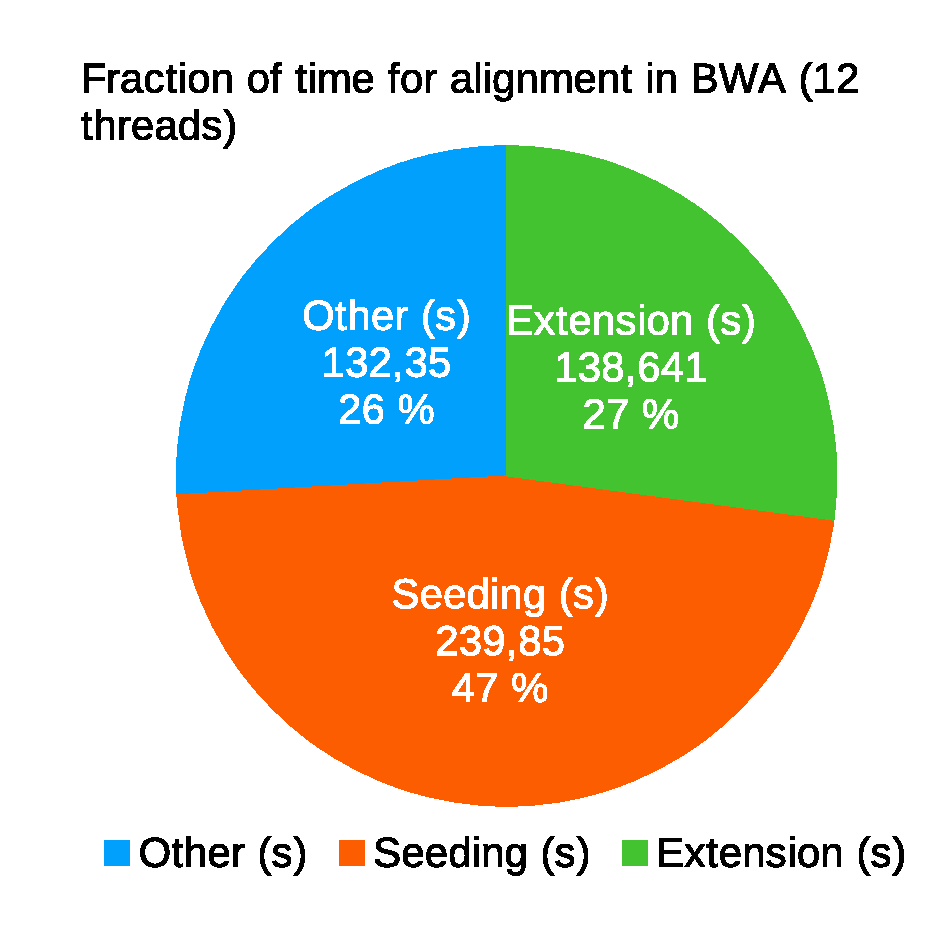
\includegraphics[width=0.65\linewidth]{bwa_time_division}
	\caption{Fraction of time for seeding, extension in an example for BWA.}
	\label{fig:bwatimedivision}
\end{figure}


\subsection{Architecture of GASAL2}
The GASAL2 library is a C++/CUDA library for DNA alignment computation. In the beginning of the project, GASAL2 was able to perform global, local and the hybrid semi-global alignment, with start position calculation. It features data compression on GPU: the goal is to quickly compress DNA strings directly in VRAM to fetch them faster when calculating the dynamic programming matrix.

Here is the list of features of GASAL2 before this thesis:

\begin{itemize}
	\item Local, global, semi-global alignment run on GPU,
	\item Operates on compressed data: there are 5 bases to describe, A, T, C, G and the unknown base N, hence needing a minimum of 3 bits to encore the base, but each based is stored on 4 bits to facilitate storing (more on this topic below)
	\item Data packing is done on GPU: despite having to transfer uncompressed data from host to device, the speed-up provided by parallel processing when packing largely makes up for the longer transfer time,
	\item Capable to reverse and, or complement any sequence on the batch independently on the GPU.
\end{itemize}

GASAL2 works with batches of sequences to align. Here, we will present the original data structure of GASAL2 before the work presented in the thesis. It revolves around a single data structure called \verb|gasal_gpu_storage_t| with the following fields, commented, on listing~\ref{lst:gpu_storage}. All fields from line 2 to 13 have their counterpart on the GPU, named the same way without the \verb|host_| prefix in their name. Since the host and the device have distinct memories, data should be handed from the host side to the device before launching computation, then the results should be retrieved from the device when it is done.  
These similar fields have been omitted for clarity, and only reminded with the comment \verb|//[copies of the abovementioned field on the GPU]|.

\begin{listing}
	\begin{minted}[
	frame=lines,
	framesep=2mm,
	baselinestretch=1.2,
	fontsize=\footnotesize,
	linenos,
	breaklines,
	frame=single
	]{C}
typedef struct {	
	uint8_t *host_unpacked_query_batch; // (string) the query sequences, butted together
	uint8_t *host_unpacked_target_batch; // (string) the target sequences, butted together
	uint32_t *host_query_batch_offsets; // array with the offsets to tell the sequences apart
	uint32_t *host_target_batch_offsets;
	uint32_t *host_query_batch_lens; // array with the length of each sequence
	uint32_t *host_target_batch_lens;
	
	int32_t *host_aln_score; // array with the alignment scores for all the sequences
	int32_t *host_query_batch_end; // array with the end position of the alignment on the query sequence
	int32_t *host_target_batch_end; // array with the end position of the alignment on the target sequence
	int32_t *host_query_batch_start; // array with the start position of the alignment on the query sequence
	int32_t *host_target_batch_start; // array with the start position of the alignment on the target sequence
	
	//[copies of the abovementioned field on the GPU]
	
	// Information about the batch
	uint32_t gpu_max_query_batch_bytes; // size of the buffer in the GPU (in bytes) for the query sequences
	uint32_t gpu_max_target_batch_bytes; // size of the buffer in the GPU (in bytes) for the target sequences
	uint32_t host_max_query_batch_bytes; // size of the buffer in the host memory (in bytes) for the query sequences
	uint32_t host_max_target_batch_bytes; // size of the buffer in the host memory (in bytes) for the target sequences
	uint32_t gpu_max_n_alns; // maximum number of sequences for the buffers on the GPU
	uint32_t host_max_n_alns; // maximum number of sequences for the buffers on the host
	cudaStream_t str; 
	int is_free; // flag to know if the computation is being run (0) or if it is finished (1)

} gasal_gpu_storage_t;
	\end{minted}
	\caption{the gasal\_gpu\_storage\_t data structure.}
	\label{lst:gpu_storage}
\end{listing}


This structure has been thought to be initialized for a given size and a given number of sequences, then have its host fields filled up with the sequences data and its metadata (length, offsets). Trying to fill more than the capacity of the fields results in a forced exit.

GASAL2 went under an important structure rework at the beginning of this thesis to drastically improve its maintainability. In the beginning, it was entirely written in plain C and had a simple architecture consisting in three files:

\begin{itemize}
	\item \verb|gasal.h|: contains all function prototypes and structure definition
	\item \verb|gasal.cu|: contains all functions code and the CUDA calls
	\item \verb|gasal_kernels.h|: contains all CUDA kernels, duplicated
\end{itemize}

Although this may seem as an easy way to split the code, it grew up to the point where it became hardly manageable. The rewrite included separating the different parts of the code in distinct files, adding interfaces for structure filling, and a class to  handle all parameters in an centralized way.

In addition, a shift to C++ has been operated to take advantage of C++ templates: they allow to produce different versions of a given function at compilation time. This will me more discussed on Chapter~\ref{chap:implementation}.

%We can draw an inclusion graph of all the files in GASAL2 in its current form. This graph is shown on Figure~\ref{fig:inclgraph}.

%\commit{Jonathan}{\today}{ADD GRAPH HERE}


 %% profiling and stuff
		
		\section{GASAL2 and the extension kernel}
		We will now review of the given architecture of GASAL2 at the beginning of this work. More details will be given on the workflow of GASAL2 and its distinctive features. Finally, we will express the list of characteristics we need for the integration.


\subsection{Typical workflow of GASAL2}

Let's describe the workflow usually followed when using GASAL2. Figure \ref{fig:dataflow} shows this flow in a graph. This flow can be instantiated multiple times from each CPU threads.

The first step is to fill the parameters used for alignment: match and mismatch scores, maximum number of sequences and maximum sizes. Then, the GPU and host storages are initialized with this given size. This step fills up the VRAM by quite a important amount because of how large the data set is. 

Then, the first available stream is selected. It is filled up with the query and target sequences and their metadata (lengths, offsets, operations for reverse/complementing if needed). Then it launches the non-blocking call for the GPU memory copies and kernel launches. These particular calls are represented in the yellow block. Note that no direct array links functions from outside the block to the inside. This is meant to show that the CPU, once making the non-blocking calls, directly jumps to the next block, and performs its large loop.

Finally, if a stream has finished, its results are retrieved. The streams system allows for full CPU-GPU overlapping calculation, allowing for important speed-up, as we will see later on.

\begin{figure}[p]
	\centering
	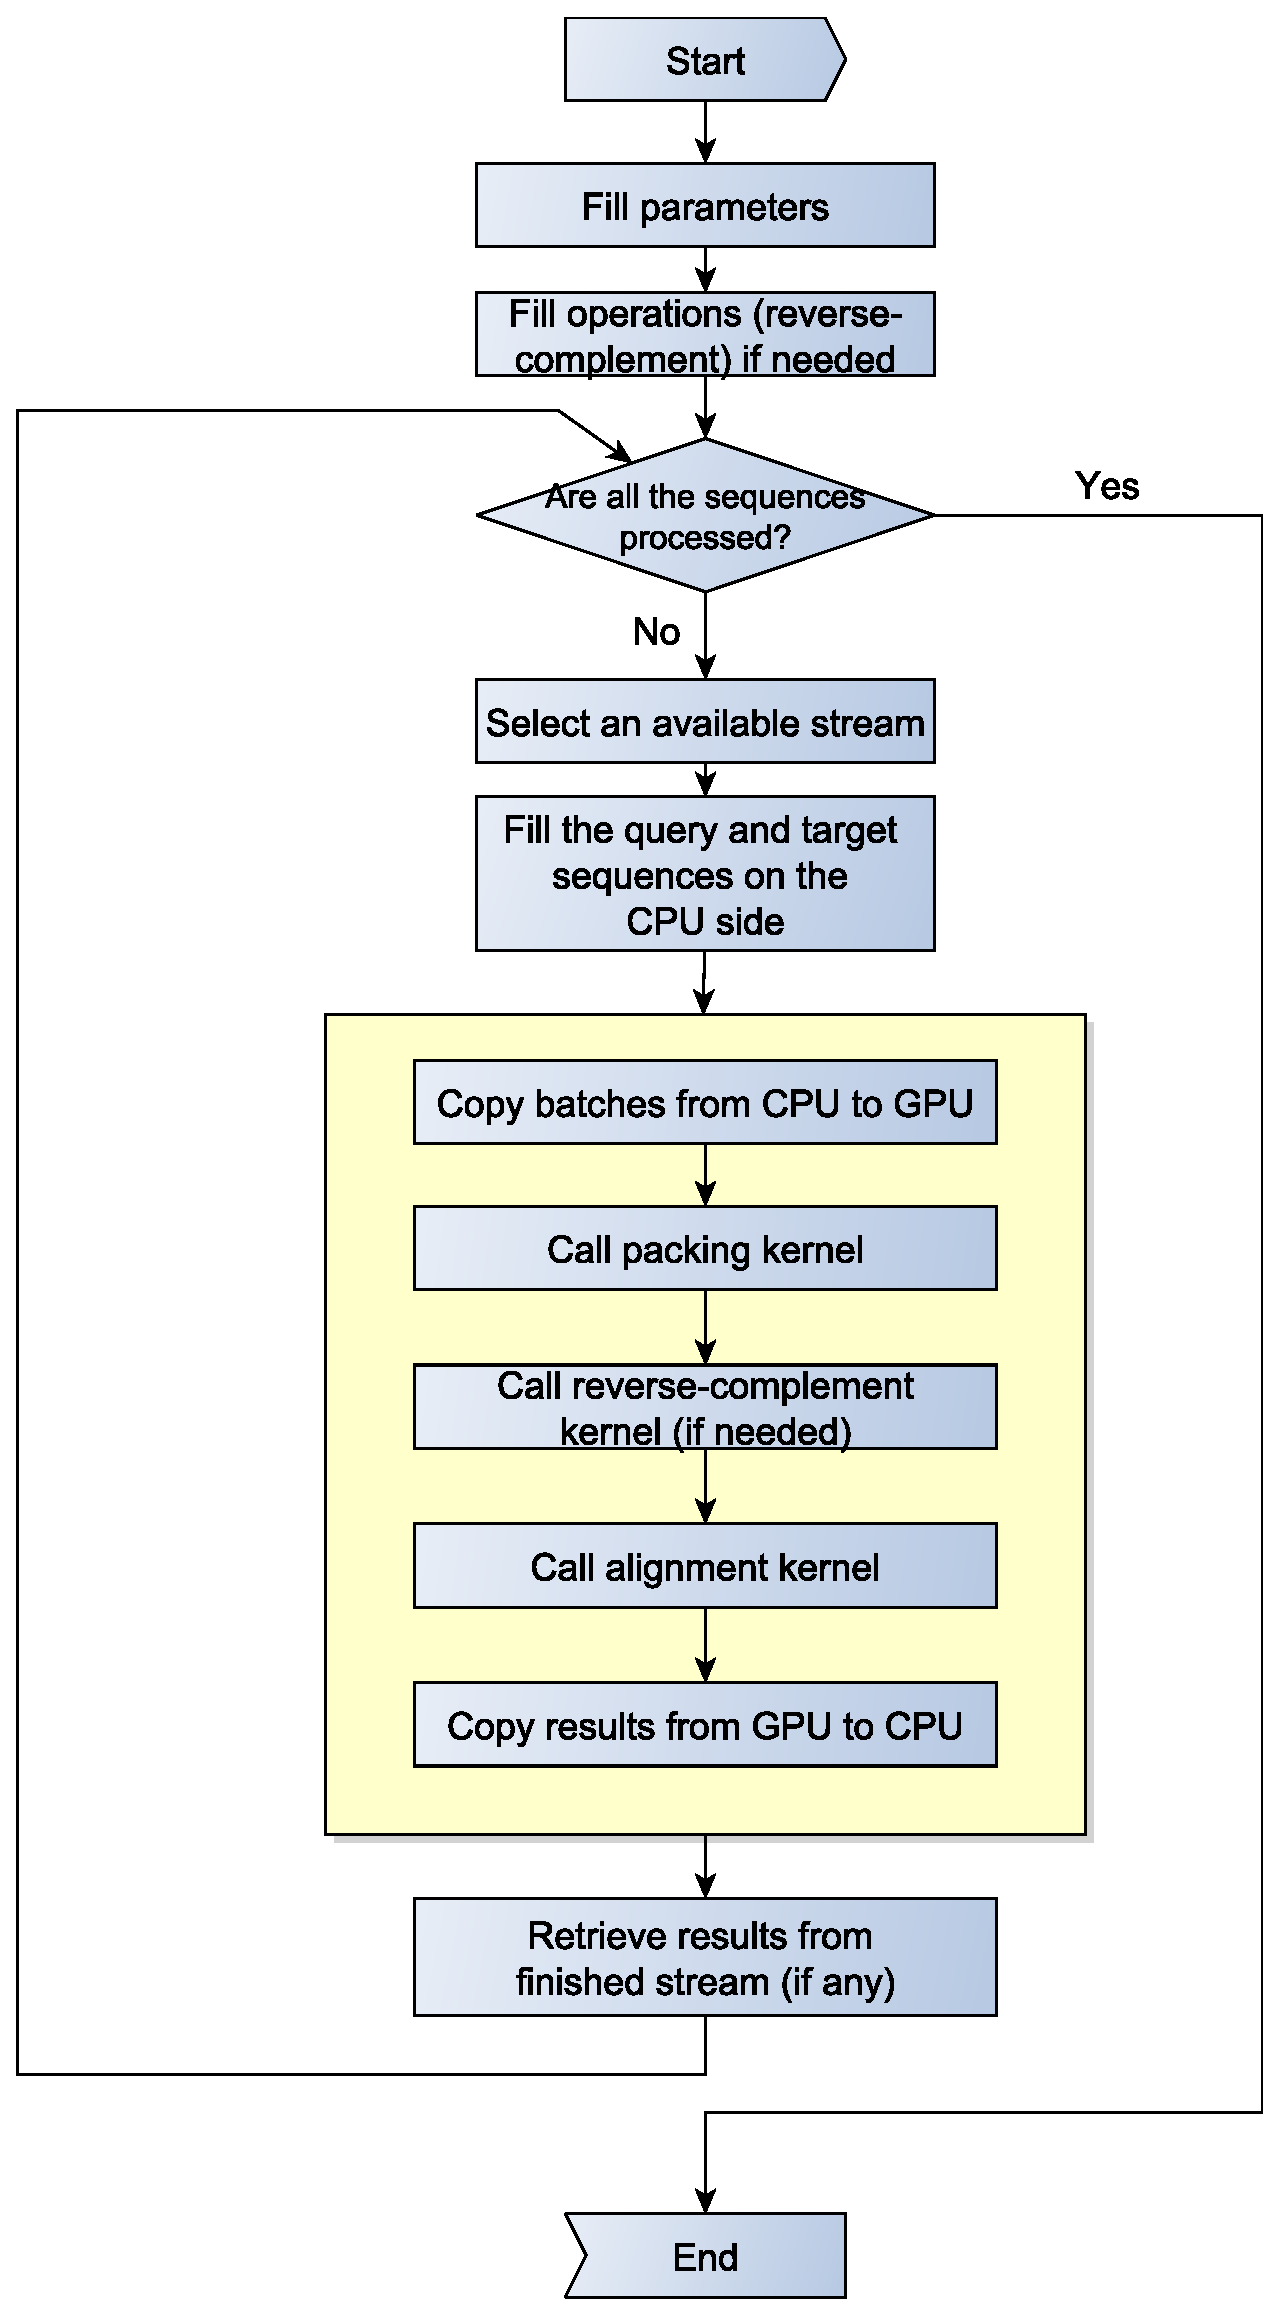
\includegraphics[width=0.85\linewidth]{dataflow}
	\caption{GASAL2 typical workflow}
	\label{fig:dataflow}
\end{figure}


%\begin{algorithm}
%	\caption{GASAL2 workflow}
%	\label{euclid}
%	\begin{algorithmic}[1] % The number tells where the line numbering should start
%		\Procedure{Align a batch of sequences}{} \Comment{}
%		
%		\While {not all sequences are aligned}
%			\State Select the first available stream
%			
%			\For {Each pair of sequences}
%				\State Copy the target sequence to the host buffer
%				\State Copy the query sequence to the host buffer
%				\State Store the length to the host array
%				\If {There is a reverse/complement operation to run}
%					\State Store the operation to the host array
%				\EndIf
%			\EndFor
%			
%			\State Select the first finished stream if any
%			
%		
%		\EndWhile
%		
%		\EndProcedure
%	\end{algorithmic}
%	\begin{algorithmic}[1] % The number tells where the line numbering should start
%	\Procedure{Launch batch alignment}{} \Comment{}
%	
%		\State Launch the copy from host to device
%		\State Launch the data packing kernel on GPU
%		\State Launch the reverse/complement kernel on GPU
%		\State Launch the alignment kernel on GPU
%		
%	\EndProcedure
%	\end{algorithmic}
%
%\end{algorithm}

An important feature of GASAL2 is that it compresses data on GPU to accelerate its handling for the alignment kernel. There are 5 different bases possible: A, T, C, G and the unknown base N. This means that a minimum of 3 bits is needed to encore 5 different values. The bases are then stores in 32-bits words. The goal is to allow the alignment kernel to fetch a pack of bases from the VRAM to operate on them directly in cache. This cache memory on a GPU is extremely small (for example, each thread has 48KB of L1 cache for the GPU in our test machine\cite{nvidia:keplerarch}), but very fast and close to the computing resources.
However, using 3 bits would mean needing a lot of bitwise operations to uncompress the data, since it would not align easily with 32-bits words. This is why the decision has been made to use 4 bits to encode the base value, hence, 8 bases are stored in each 32-bit word. This way, the kernel fetches two 32 bits words (one for query, one for target) and can easily uncompress the 8 bases stored. The dynamic programming matrix is then computed by tile of 8 by 8 bases.


\subsection{Characteristics of GASAL2 launches}

The kernel launch has adaptable parameters to tune it for a given data set, a given CPU thread number and a given GPU thread number. In its current state, there are up to three different types of kernels to run:

\begin{itemize}
	\item the packing kernel
	\item the reverse/complement kernel, if needed
	\item the alignment kernel (be it local, global, or else)
\end{itemize}

The packing and the reverse/complement kernels are very low in computation, and take almost no time to complete compared to the alignment kernel. With various data sets, for the given machine on which this work has been coded and run, it has been measured that the packing kernel takes at most 0.6\% of the kernels run times, and the reverse/complement kernel takes at most 4\% of the kernels run times when all sequences must be both reversed and complemented, and data transfer time take at most 4\% of the total time. Note that these times are given here as a rough estimate to show the importance of some tasks compared to others, and that precise measurements are presented on Chapter \ref{chap:measurements}. As expected, the large majority of the time is taken by the alignment kernel.

This kernel has a variable GPU occupation depending on the data processed. On our test machine, with a single thread, the GPU occupation oscillates between 3\% and 10\%. Even though it seems a very low occupation, it is not a major problem since GASAL2 can be spawned from multiple threads, multiplying the occupation by the same number and allowing to get closer to 100\%.


\subsection{Extension kernel behaviour}
\label{sec:seedonly}
The aim of this project was to integrate GASAL2 in BWA to perform the extension part. To do this, we need to reproduce the behaviour of the extension kernel of BWA to replicate it in GASAL2.

The original extension function has a BLAST-like behaviour. It starts from a pair of target and query sequences, knowing the position of the beginning of the seed, its length, and its score, then proceeds as follows:
\begin{itemize}
	\item it isolates the left part of both sequences, and reverse it.
	\item it computes a local alignment with the beginning score equal to the seed score. The end position of this alignment is equal to the beginning of the alignment of the two sequences (the alignment progresses from right to left, since the left parts have been reversed)
	\item it then isolates the right part of both sequences,
	\item it computes a local alignment with the start score equal to the left score previously computed (which includes the seed score).
\end{itemize}

In our case, this approach is unpractical because one would like to compute both sides in parallel to maximize GPU use. In this fashion, we do not have other choices than making both extensions (left and right) start with a score equal to the seed score, which could make a small difference in the final result. We expected this error between the regular BLAST-like computation and our slightly different approach to be small enough to consider this approach valid. We effectively measured it after implementation, with results shown in chapter \ref{chap:measurements}. We reached the conclusion that the difference was effectively very small and that calculating both sides at the same time only using the seed score is an acceptable way to solve this problem. We call that paradigm the "seed-only" method.

Another problem comes from the rigidity of GASAL2 memory scheme. Originally, GASAL2 was not able to scale in memory and adapt if some sequences were longer than expected, resulting in a crash of the program. This is particularly problematic when integrating it in BWA, because the number of seeds is unknown in advance, so each batch in GASAL2 need to have a variable size; plus, left and right parts to align have an unpredictable length. 
An extensible data structure should be implemented to tackle this issue with minimum overhead.


	
		
		\section{Proposed CUDA kernel}
		With the informations we unfolded up to now, we would like to design a library interface with a kernel that complies with the following technical specifications:

\begin{itemize}
	\item The library should be able to start with any amount of memory and extend it whenever needed. Moreover, the memory allocations should remain as scarce as possible.
	\item The kernel should reproduce the behaviour of BLAST-like kernels by allowing local DNA alignment with a non-zero starting score.
	\item The interface on BWA side with the library should approach the behaviour of BLAST-like alignment by calling the kernel and retrieving the alignment scores in the "seed-only" fashion, as explained on section~\ref{sec:seedonly}.
	\item The end product should be readily available with as an open-source project, respectful of the original licenses, and with a complete traceback of the code production.
\end{itemize}

With the specification written, now we have to state the goals and metrics used to verify that the end product meets the bill of specification, that is, that its behaviour meets the following expectations: 

\begin{itemize}
	\item The integration of GASAL2 in BWA should effectively speed up the alignment process. We will compare the kernel execution times before and after acceleration, in seconds. We will also compare the total execution time, to check the difference that hidden-time execution makes.
	
	\item Using the seed-only paradigm should not bring any difference to the vast majority of the alignments. Still, there is no guarantee that the results will be exactly the same. Whenever the alignment differs, the difference with the original BLAST-like paradigm should be minimal. Result correctness will be carefully examined. We will quantify the number of differences between the two results output from BWA and its accelerated version, for our given data sets.
	
	\item The VRAM use should not take more than what it necessary. To verify this, we will take advantage of the feature that should allocate more VRAM when necessary to purposefully initialize the \verb|gpu_storage| structure with a small size and let it grow bigger to just the right amount. This will give us a lower bound that will be by construction close to the actual VRAM usage needed for our data sets.
	
\end{itemize}

In the next chapter, we will detail the choices we made to meet the technical specifications.
	
	\chapter{Implementation}
	\label{chap:implementation}
	In this chapter, we will review the choices we made for the implementation of the features discussed earlier. We will focus on what feature is implemented, how it was written, and why we chose to implement things the way they are. Although some code snippets are provided, a closer look to the program as a whole~\cite{j-levy:bwa-gasal2} can be helpful to understand the coupling between different parts of the software.
		
		\section{C++ Kernel templates}
		
\subsection{Factorize kernel codes with templates}

During the refactoring of the library code, we had to factorize the code from very close kernels. It would not have been maintainable to keep multiple kernels extremely similar. However, it is not viable to directly make a generic kernel with \verb|if - then - else| conditions inside, since it would create a major slowdown. This is because GPU execution runs the same instructions for all threads in an ensemble of threads called warp. For most NVIDIA GPUs, warps are made of 32 threads. Introducing conditions would make a divergence between the threads in the warp, creating different contexts and not running threads concurrently.

The solution we adopted consists in using C++ templates to generate multiple specialized version of a kernel at compilation time. We can then write branches in a clean fashion that would be resolved by the compiler. However, we cannot make any conditions on integer values from the get-go: since templates are resolved at compilation, the compiler can only resolve symbols on classes and types, and not values. 

We then use a small template as shown on listing~\ref{lst:tmp} to derive our own types from integer values. We first define a template structure \verb|Int2Type| with inside an enumeration with a single value, equal to the one given for its template instantiation. The goal is to instantiate empty structures which are seen distinctly by the compiler. Hence, at compilation time, \verb|Int2Type<0>| is a structure name, \verb|Int2Type<1>| is another structure, and so on.

We then create a template structure \verb|SameType| that can be instantiated in two ways: if two objects of different types are passed (line 5), it bears an enumeration with value 0, and if types are the same (line 9), it bears value 1. Writing \verb|if| blocks using the \verb|SAMETYPE(a, b)| macro will expand it into 0 or 1, allowing the compiler to prune the unused branch automatically.

\begin{listing}[h!]
	\begin{minted}[
	frame=lines,
	framesep=2mm,
	baselinestretch=1.2,
	fontsize=\footnotesize,
	linenos,
	breaklines,
	frame=single]{C++}
template <int Val>
struct Int2Type{
	enum {val_ = Val} dummy;
};
template<typename X, typename Y>
struct SameType {
	enum { result = 0 };
};
template<typename T>
struct SameType<T, T> {
	enum { result = 1 };
};
#define SAMETYPE(a, b) (SameType<a,b>::result)
	\end{minted}

	
	\caption{Meta-programming template to derivate types from integer values}
	\label{lst:tmp}
\end{listing}
	
Finally, for all the kernels to be generated, explicit calls must be written in the source code. We decided to group all the kernels in three major kernel templates. Each of them can specialize to various extent:

\begin{itemize}
	\item global, that does not have any specialisation,
	\item local, on which we can select among 4 combinations:
	\begin{itemize}
		\item start position calculation (on / off),
		\item second-best score calculation (on / off);
	\end{itemize}
	\item semi-global, on which we can select among 64 combinations:
	\begin{itemize}
		\item if we allow to skip the beginning, the end, both ends or none of the ends of either query or target (making it 16 different cases),
		\item start position calculation (on / off),
		\item second-best score calculation (on / off).
	\end{itemize}
\end{itemize}

It would be highly unpractical to list all these variations, but we had to have them written before the compilation phase, where the templates are resolved. Subsequently, we rely on the C++ preprocessor and used a series of macro expansion to develop a \verb|switch - case| including all variations. This allows to write each kernel call exactly once, and condense all calls in a clean way.

\subsection{Porting newer version of GASAL2 in GASE-GASAL2}

Several modifications to BWA were done to integrate GASAL2 for its extension step. While some of them were already done when starting this thesis, there was an important amount of changes to successfully integrate it. In particular, the system to process sequences in pack was already implemented in a custom version of BWA for measurements called GASE-GASAL2~\cite{Ahmed:gase-gasal2}~\cite{Ahmed:GASE}. For the recall, GASAL2 works with batches of sequences to align, and with a given batch of $k$ alignments, it instantiates $k$ threads that run the alignment kernel on the GPU. This behaviour is intrinsic to how GPU computing works: in fact, we need to run a given kernel, hence complete a given task, on all the parts of a large data set, so we need to provide a batch of data to process in parallel.

This piece of software called GAS-GASAL2 only uses GASAL2 as local aligner and does not provide accurate scores that can be compared with BWA. It has only been developed as a demonstrator of how alignment could be accelerated. It used an old version of GASAL2 which became incompatible with the changes we made previously.

The first task has been to update GASE-GASAL2 to compile it with the newer version of GASAL2. In particular, the source code had to be ported to C++. Several wrong writing practices had to be fixed, including naming variables "or" (which is a keyword in C++), and defining clear context for function prototypes in the header files. In fact, C++ features name mangling for functions, which adds context information at compilation to establish contexts where function names are declared valid. This feature is implemented among others for function overloading. Unless plain C functions are placed in \verb|extern 'C' { ... }| blocks, they cannot be resolved at compilation, inducing a linking error, so some code clean-up had to be done on this side.
	
		\section{Kernel implementation}
		Let's review with the kernel implementation.

\subsection{Kernel writing}
The kernel in itself is written in CUDA in the GASAL2 library. It should exactly replicate the behaviour of the original function in BWA, called \verb|ksw_extend|. From there on, we will refer to the original function with this name, and to its GPU implementation as the \verb|ksw_kernel|.

We have seen before that previous kernels in GASAL2 were written as C++ template functions. It has been considered using the already existing local alignment kernel template to derivate an alternate kernel with the starting scores. This could have reduced the amount of code to maintain. However, the more we investigated this possibility, the more differences we found out between the to-be seed-only kernel and the local kernel we had. In particular, an important number of speed-up were present in \verb|ksw_extend| and marked a high level of difference with the previous solution. For the sake of simplicity, we created a new kernel dedicated to the seed-only paradigm.

The kernel has been built by copying the original \verb|ksw_extend| and renaming the variables to plug it into the naming convention used in GASAL2 kernels. At first, we followed the loop structure used in \verb|ksw_extend|in which there is no data compression. The behaviour is simply to fetch the current base from query and the current base from target and calculate the cell of the dynamic programming matrix. Therefore, the pseudocode is the same as presented previously in algorithm~\ref{algo:local}.

Secondly, we introduced the use of compressed data by fetching the 8 bases in the 32-bit words from query and target. This added two innermost loops in the algorithm to perform the alignment tile by tile, using square tiles of $8 \times 8 = 64$ bases.

Because of memory constraints, the whole matrix is not stored in memory. Instead, only a full row having the length of the query string is stored. For the record, only the north, west, and north-west cells are needed for the computation. This is shown on figure~\ref{fig:visualization-aid-tile}. The cells are computed in the order given by their number. When a full column is computed, the orange column moves one step on the right, taking the place of the cells numbered 1 to 8, then cells 9 to 16 when they are computed, and so on. This column is the western cells used to compute the score. When all cells in the tile are computed, the 8-cell setion of the yellow row moves 8 cells down, taking the place of the cells numbered 8, 16, 24 ... 64. When the cyan tile is computed, it goes to the blue one, then the navy blue, then the next line.

\begin{figure}[h!]
	\centering
	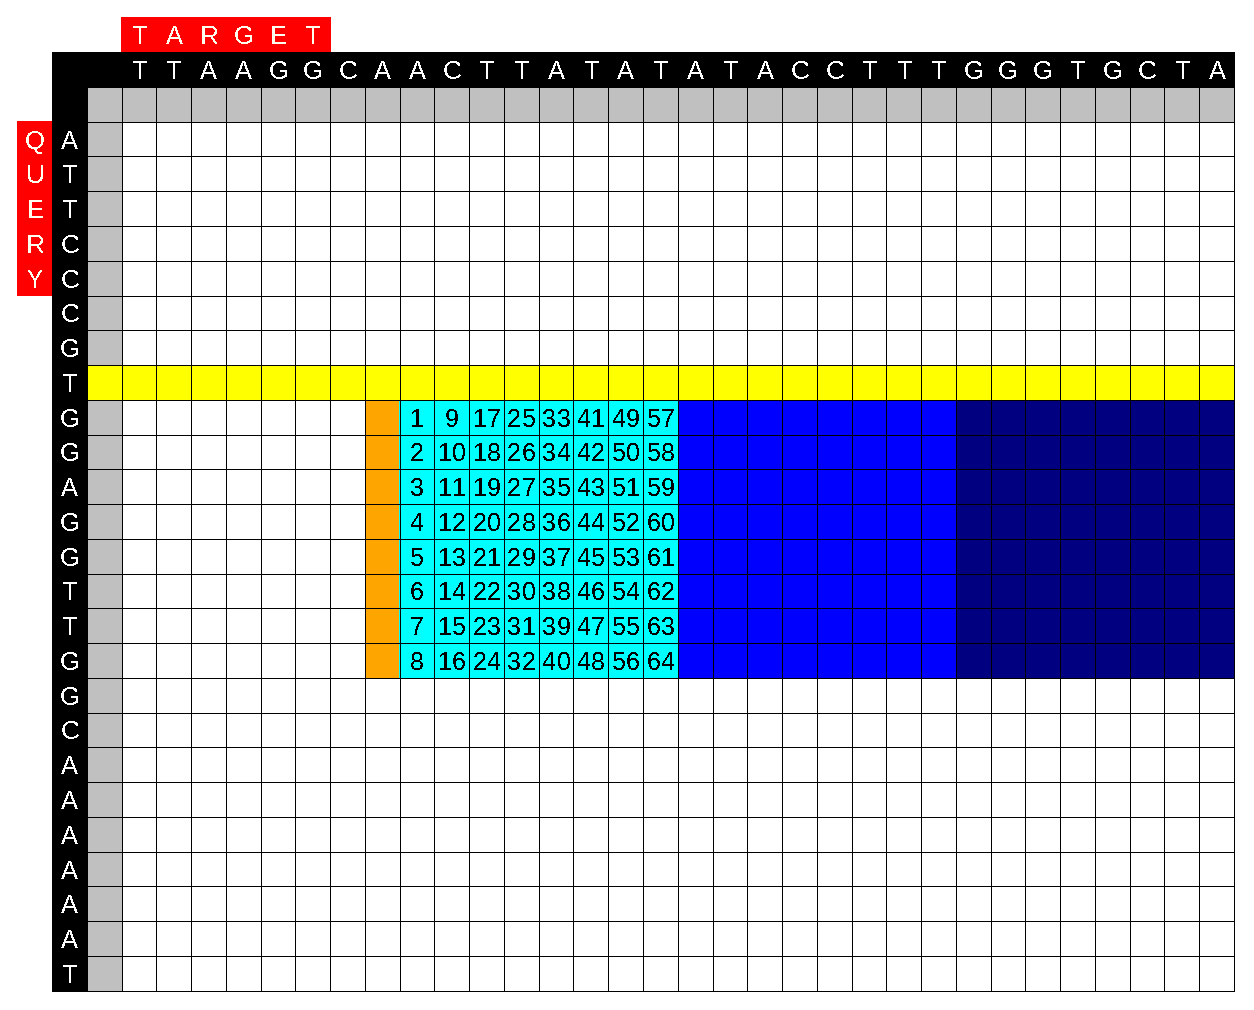
\includegraphics[width=0.9\linewidth]{visualization-aid-tile}
	\caption{Visualization of the tile-based matrix computation. Only the yellow row and the orange column are stored in memory.}
	\label{fig:visualization-aid-tile}
\end{figure}

The algorithm change as shown in ~\cite{Ahmed:gasal}.

Finally, we introduced again some computing optimization that we disabled in the second version of the kernel, in particular, z-dropoff. This optimization allows to skip the calculation of some cells of the matrix provided the score drops below a certain threshold. When this happens, it usually means that the alignment will not improve because the difference between the two sequences grew too big, so it is usually better to stop computing altogether instead of wasting time trying to align two sequences that are visibly very different.

\subsection{Score comparison}

To verify the correctness of this implementation, a modified version of BWA is made from the original BWA~\cite{lh3:bwa}. This version is hosted on GitHub~\cite{j-levy:bwa} and has different branches to switch from one behaviour to another, to compare the results with the GPU-accelerated implementation.

In a branch called \verb|no-zdrop-seedonly|, we introduced our seed-only method instead of the original BLAST-like behaviour. As the name suggests, we also disabled the z-dropoff when comparing the result for this branch, but we re-introduced it afterwards to check the implementation of the z-dropoff in GASAL2, and verified that they matched.

The results are in the Sequence Alignment/Map (SAM) format, commonly used for DNA alignment. SAM is text-based, extensively documented~\cite{samtools:sam} and widespread among DNA-related programs. It is the default format output for BWA. Using \verb|diff| and other regular UNIX tools, we can compare the number of lines that differ between the reference program and a modified version. Knowing the original number of lines, we can draw out a percentage of difference between the files, as shown on listing~\ref{lst:diff}.

\begin{listing}[ht]
	\begin{minted}[
	fontsize=\footnotesize,
	linenos,
	breaklines,
	frame=single]{bash}
#!/bin/bash
DIFFLINES=$(diff --suppress-common-lines --speed-large-files -y $1 $2 | grep "[|><]" | wc -l)
TOTALLINES1=$(cat $1 | wc -l)
PERCENTDIFF=$(bc -l <<< "scale=2; (100*$DIFFLINES)/$TOTALLINES1")

echo "Different lines between " $1 " and " $2 " = " $DIFFLINES
echo "Total numer of lines in" $1 " = " $TOTALLINES1
echo "Difference = " $PERCENTDIFF "%"
	\end{minted}
	\caption{Bash script to show percentage of difference between two files}
	\label{lst:diff}
\end{listing}


		
		\section{Library integration}
		After the C++ adaptation of GASE, the demonstrator for BWA-MEM and GASAL2 integration, we obtained a valid version of BWA-MEM processing sequences in batches, originating from GASE-GASAL2.

BWA-MEM operates with the seed-and-extend paradigm, and GASAL2 can run the extension part. For a single query sequence, a variable number of seeds can be found. 

For every seed found in the query, the target sequences is the region in the genome around the seed location. The extension step is then either:

\begin{itemize}
	\item skipped, meaning that the seed is exactly the size of the sequence,
	\item or done only on one side, if the seed is located at the beginning or the end of the query sequence,
	\item or done on both sides, if the seed is in the middle of the sequence.
\end{itemize}

Most of the time, both sides have to be extended. We create two GPU batches. A simple approach would be to define a batch for the left side, and one for the right side. However, there is an optimised way to split the alignments between two batches.

GPU threads are grouped in \emph{warps}. All threads in a warp run the same instructions. For maximal performance, it is advisable to run as many grouped thread as possible, and avoid differences in execution causing \emph{thread divergence}. To avoid this thread divergence, sequences aligned by the GPU threads in the same warp should have similar lengths. But if one seed is located on the far left and another one on the right, knowing that all queries have the same length, the left parts of the extension will have very different lengths, as shown in Figure~\ref{fig:seds-different-chains}. Moreover, the processing time will be limited by the length of its longest alignment in the GPU batch.
\begin{figure}[h!]
	\centering
	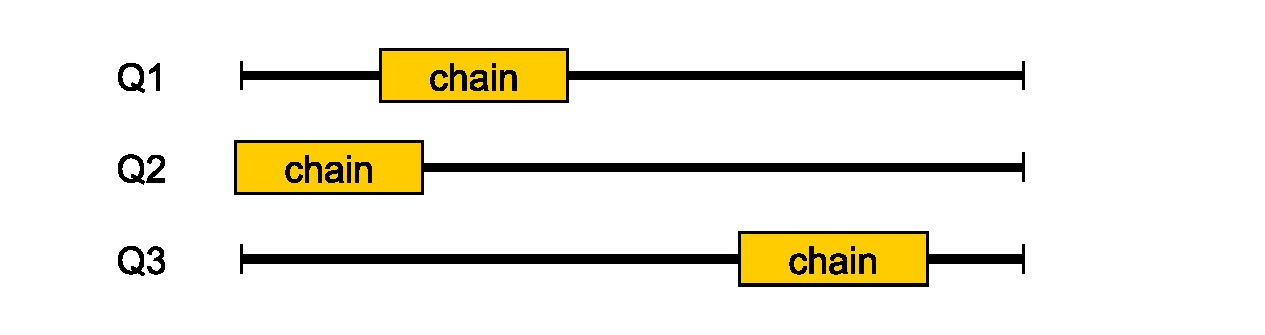
\includegraphics[width=0.7\linewidth]{seds-different-chains}
	\caption{Illustration of chains (in yellow) being located on different places}
	\label{fig:seds-different-chains}
\end{figure}

To summarise, we note that :
\begin{itemize}
	\item all reads have the same length,
	\item the final score is equal to the sum of the chain score, the left part score, and the right part score,
	\item to that extent, we don't need to know whose score is the left one and the right one (only the sum matters),
	\item and we would like to process both sides in parallel.
\end{itemize}

So instead of using two batches for left and right extension, we use two batches for long and short extension. This puts the long sides together to minimise thread divergence. The difference between the longest and the shortest extension in each batch is now at most half the length of the query sequence. For each chain, we log in a dedicated data structure if it has zero, one or two alignments, and on which part (left or right) the long alignment is. When both the "long" and "short" batches of extension are done, the scores are gathered.

Another problem arises: the seeds may have zero, one or two extensions, the short and long batches can have a different number of extension to make. To show this with an example, we can assume that we have three seeds as in Figure~\ref{fig:seds-different-chains}. For the sake of conciseness, only query sequences have been shown, but assume each of these queries have a corresponding target sequence with the same seed located in it, forming pairs of query-target sequences. Chains from Q1, Q2 and Q3 are found in this order, and the \verb|gpu_storage| structure is filled in this order too. Table~\ref{tbl:batches} shows how the batches are filled for this case. Notice that the number of sequences are not the same in two batches, hence two sides of the same alignments are not at the same index on both structures. To circumvent this problem we added information in the data structure of BWA-MEM that contains the alignment scores. After both sides of the seed-extension of a batch are finished, this data structure is used to know how many alignments (0, 1 or 2) for a seed were computed, ensuring correct gathering. This is not an issue in the original software as the seed is extended first to the right and then to the left. But in our implementation we run both the extensions in parallel, with seed score as the starting score of the alignment, to get more parallelism. Hence, if we sum both left and right scores, we count the seed score twice. Therefore, we subtract the seed score from the total of extension scores of left and right side. When only one extension is made (or none), we do not have to do this subtraction.

\begin{table}
	\centering
	\begin{tabular}{|c|c|}
		\hline 
		\textbf{``Long" batch} & \textbf{``Short" batch} \\ 
		\hline 
		Pair 1, right part & Pair 1, left part \\ 
		\hline 
		Pair 2, right part & Pair 3, right part \\ 
		\hline 
		Pair 3, left part &  \\ 
		\hline 
	\end{tabular} 
	\caption{Example of how batches are filled.}
	\label{tbl:batches}
\end{table}


		
		\section{Memory management}
		For GASAL2 to work correctly, all data fields in the \texttt{gasal\_gpu\_storage\_t} structure must have their sized specified at initialization. This is problematic with BWA because sizes cannot be inferred beforehand. Even if we process a pack of 4000 sequences, each of them have an unpredictable number of chains. Furthermore, for each chain, the length of the query and target parts that have to be aligned are unknown too. We show a schematic view for this problem on figure~\ref{fig:cpu-gpu-batches}. BWA processes query sequences by packs. On the picture, they are packs of 3 sequences (note the sequence numbers on the left). For each of them, they can have different number of seeds. The pack is split equally between sequences (this is difficult to show with a few number of sequences like here, but for example, a pack of 4000 sequences is split into 4 GPU batches of 1000 sequences each). All seeds extensions of a given sequence are processed in the same batch. Alignments of the same colour are processed in the same GPU batch. We can see that the total number of alignment is different depending on the number of chains, and each alignment has its own left and right lengths.

\begin{figure}[h!]
	\centering
	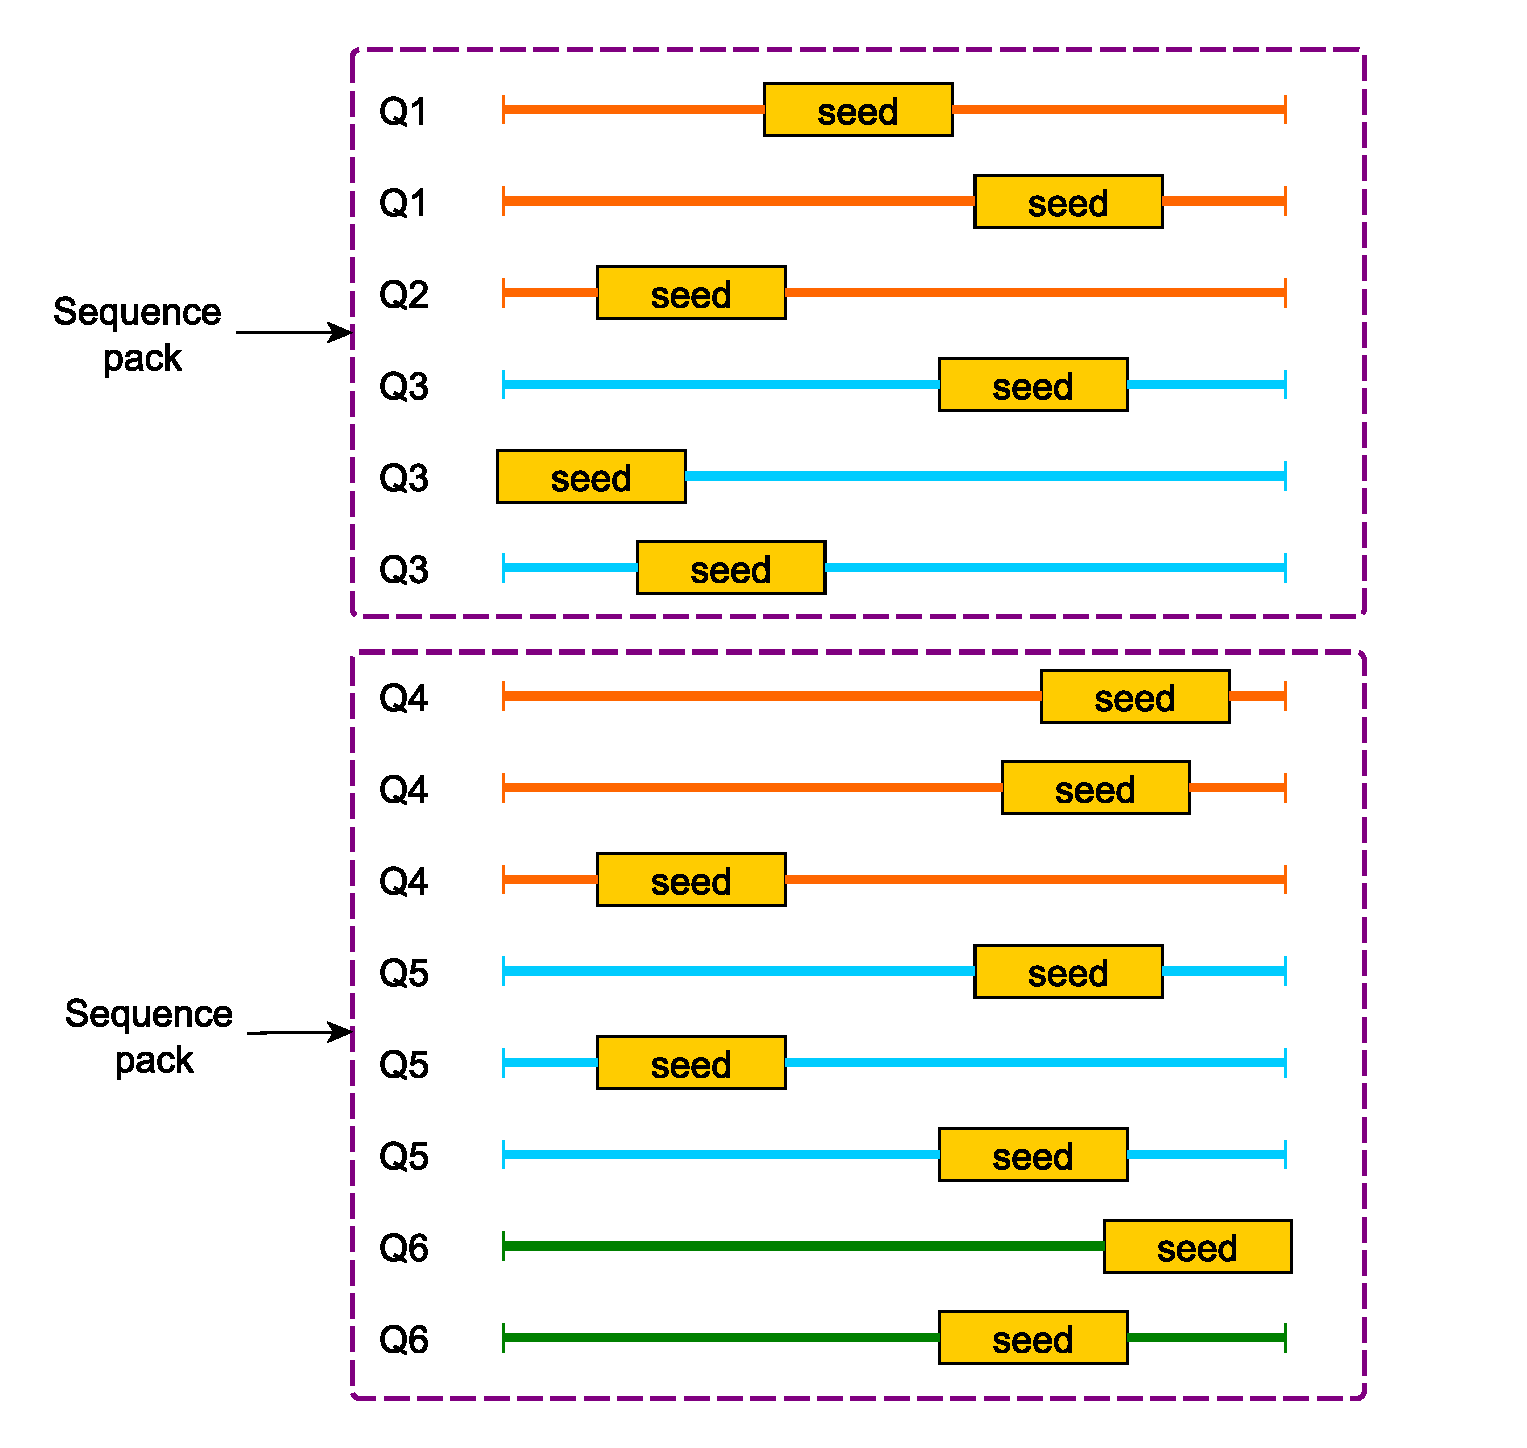
\includegraphics[width=1\linewidth]{cpu-gpu-batches}
	\caption{Representation of alignment distribution in sequences packs across GPU batches.}
	\label{fig:cpu-gpu-batches}
\end{figure}


We would need some automatic resizing whenever the size gets insufficient.
For a given data set, during testing phase, we can estimate a higher bound to allocate in the program source code. But this is not , since we have to allocate much more memory than actually required.

In this section we will review the solutions we implemented. A simple approach was adopted for all the arrays carrying metadata for the sequences. We chose a more refined approach for the fields bearing the actual sequences to minimize overhead caused by reallocation.

\subsection{Memory reallocation for arrays fields}

A large number of fields in the \verb|gasal_gpu_storage_t| are containing information about the sequences entered. These fields are arrays of length equal to the number of sequences. As such, they do not store a very large amount of data, and their separation is clear (each slot of the array is holding information about one single sequence). For example, we need to store the length of each query and target, the offset of each each query and target, and so on. These fields are first allocated on host side, then they are copied onto the device, so they are allocated with \verb|CudaHostAlloc|. Since there are a lot of them and they do not represent a major part of memory allocation, we decided to implement a simple realloc feature for all fields. This function is displayed on listing~\ref{lst:cudarealloc}. Note that on the \verb|gasal_gpu_storage_t| shown on listing~\ref{lst:gpu_storage}, all fields do not have the same type: some are of type \verb|uint32_t|, others are \verb|uint8_t|, and so on. We made a simple use of C++ template to adapt this function to multiple types. It allocates a new memory area, copies the content of the former area, and frees it. It returns a pointer to the newly allocated area in memory filled with the previous data. This re-allocator is called by a bigger function resizing all the necessary fields when the number of sequences filled exceeds the number of maximum sequences the structure can hold.

\begin{listing}[h!]
	\begin{minted}[frame=lines,
	framesep=2mm,
	baselinestretch=1.2,
	fontsize=\footnotesize,
	linenos,
	breaklines,
	frame=single]{C++}
// Function for general resizing
template <typename T>
T* cudaHostRealloc(void *source, int new_size, int old_size) 
{
	cudaError_t err;
	T* destination = NULL;
	if (new_size < old_size)
	{
		fprintf(stderr, "[GASAL ERROR] cudoHostRealloc: invalid sizes. New size < old size (%d < %d)", new_size, old_size);
		exit(EXIT_FAILURE);
	}
	CHECKCUDAERROR(cudaHostAlloc(&destination, new_size * sizeof(T), cudaHostAllocMapped));
	CHECKCUDAERROR(cudaMemcpy(destination, source, old_size * sizeof(T), cudaMemcpyHostToHost));
	CHECKCUDAERROR(cudaFreeHost(source));
	return destination;
};
	\end{minted}
	\caption{Reallocation function for CUDA allocated fields.}
	\label{lst:cudarealloc}
\end{listing}

With the progress currently made, the programmer in charge of integrating the library must take care of the sequence count and run the resizer when needed. Once the fields are reallocated to a bigger memory area, they keep their new size, so they don't need to be re-allocated until the next time the new maximum capacity is exceeded. The structure can store the current number of sequences filled into it, and the maximum number. 

We chose a different approach for the actual sequences because of their bigger size, making them much longer to reallocate.

\subsection{Extensible data structure for sequences}

Using the same reallocation for the sequences could have been possible, but unpractical. In fact, these memory allocations and frees are costly in time. While this is reasonable for smaller arrays having only 4-bytes elements (like \verb|uint32_t|), it takes too much time with the sequences arrays. The query and target fields are storing all the DNA strings butted together (one field for all queries, the other for all targets). In terms of space taken, on BWA, if a pack of 1000 sequences is processed, it can require between 10 000 to even 100 000 chains, making it up to 200 000 alignments to proceed (most chains needing both left and right extension). Each base being stored on one byte, it makes these fields 20 to 30 times bigger than the others.

For this issue, we designed a structure of linked list to allocate more and more memory progressively without needing to move around already existing data. This structure shown on listing~\ref{lst:extensiblehostbatch} starts with a single element and each of them carries some metadata about its content size to ensure correct filling. It stores:

\begin{itemize}
	\item the sequences, butted together, in the field \verb|*data|,
	\item how many bytes are already stored, in field \verb|data_size|,
	\item the total size available in bytes, in the field \verb|page_size|,
	\item the data \verb|offset|, which is equal to the data size of the previous element of the linked list,
	\item A flag telling is the structure can store new data or not, \verb|is_locked|, set to 0 or 1,
	\item and of course, as for all linked list, a pointer to the next element.
\end{itemize}

\begin{listing}[h!]
	\begin{minted}[frame=lines,
	framesep=2mm,
	baselinestretch=1.2,
	fontsize=\footnotesize,
	linenos,
	breaklines,
	frame=single]{C++}
struct host_batch{
	uint8_t *data;
	uint32_t page_size;
	uint32_t data_size;
	uint32_t offset;
	int is_locked;
	struct host_batch* next;
};
typedef struct host_batch host_batch_t;
	\end{minted}
\caption{The linked list structure for sequences on host.}
\label{lst:extensiblehostbatch}
\end{listing}

The sequences are filled by a dedicated function from GASAL2 that takes care of allocating more memory if needed. This function takes as input the sequence to add, the storage structure, and if it is a query or target sequence to fill, and operates with the algorithm shown on algorithm~\ref{algo:extensiblefunction}. We represent the fields belonging to an element with the symbol $\rhd$, like the symbol \verb|->| is used in C++ to get the field belonging to a pointer to a structure.


\begin{algorithm}[h!]
	\caption{Behaviour of the sequence filler function}
	\label{algo:extensiblefunction}
	\begin{algorithmic}[1] % The number tells where the line numbering should start
		\Function{Fills one sequence in an linked list }{$gasal\_gpu\_storage\_t$, $seq$, $seq_length$, $seq_offset$, $data\_source$}
		
		\State Select query or target linked list from $data\_source$
		\State Select first non-locked linked-list element, $~e$
		\State Compute padding length $padding\_length$
		\State $total\_length \leftarrow padding\_length + seq\_length$
		
		\If{$e$ is the last element \textbf{and} $total\_length \geqslant e\rhd page\_size - e\rhd data\_size$}
			\State Create new\rhd element twice as big
			\State Append it to the last element $e$
			\State Select last element (newly added) of the linked list, define it as $e$
		\EndIf
		
		\If{$e$ is not the last element \textbf{and} $total\_length \geqslant e\rhd page\_size - e\rhd data\_size$}
			\State $e\rhd next\rhd offset \leftarrow e\rhd offset + e\rhd data\_size $
			\State Mark $e$ as locked
			\State Select next element $e\rhd next$ of the linked list, define it as $e$
		\EndIf
		
		%\If{$total\_length \leqslant e\rhd page\_size - e\rhd data\_size$}
			\State Store the sequence in $e\rhd data$ add the padding
			\State $e\rhd data\_size \leftarrow e\rhd data\_size + total\_size$
		%\EndIf
		
		
		\Return $offset$
		\EndFunction
		
	\end{algorithmic}
\end{algorithm}

In the beginning, the first non-locked element is selected. Then the algorithm operates in three main steps. 

\begin{enumerate}
	\item First (line 6), it checks if the selected element is the end of the chain, and if there is not enough space in it. If so, the only solution is to create a new element to append at the end of the chain.
	\item Then (line 11), it checks if there is more elements down the chain, but if the current element is full. This happens when the chain has been creating new elements during previous fillings and kernel launches. We already selected the first non-locked element so it is full, we simply jumps to the next one, and lock the previous one so that we don't try to fill it anymore (it is full).
	\item At this point (line 16), we have reached an element who must have enough free space for the sequence (either by having an element available from the beginning, or we filled the current available one so we locked it and moved to the next one, or we created a new one), so we fill it with the sequence and its offset.
\end{enumerate}

At the end, the function returns the current offset, corresponding to the number of bytes totally present in the linked list, which is needed to continue the filling for the next sequence.

In the end, we can end up with a linked list which is filled by full sequences. In other words, for the sake of not splitting the sequences between two elements, we do not exactly fill each element up to its maximum capacity. 

When copying the batches onto the device, all elements are processed using \verb|CudaMemCpy|. The size to copy is directly given by the field \verb|data_size|. At this moment, all the elements in the linked list are set as "non-locked". This way, they can be re-used for future launches. The linked list can only grow in size, and always grows ever bigger to minimize the possibility of having to do another allocation later on. This is why we implemented this "locked" flag to get the information if the element has been filled for the current batch, to know where to start filling up.

All in all, this allocation scheme allows to get more memory space without moving around already existing data, always re-use all the previously created memory chunks in the linked list, and creates bigger and bigger elements to lower the probability of having to allocate a high number of them.

%\vspace{0.1\textheight}
\section*{Wrap-up}
In this chapter, we reviewed all the modifications and new implementation we carried out to successfully integrate GASAL2 in BWA. We started from a demonstrator already presenting the processing in pack of sequences, and we first ported it to C++ to run it with the newer version of GASAL2. We created a CUDA kernel that replicates the behaviour of the original C function in BWA. We integrated the library with our "seed-only" paradigm to tackle the issue of processing both sides of the extension at the same time, which created its own issues with score synchronization between left and right sides, that we addressed. The memory management is now done with a reallocation in number of alignments, along with a linked list of elements for the actual data to minimize the number of memory operations. Finally, we tested this implementation in our hardware with a sample data set, that we will present in the next chapter.



	
	\chapter{Measurements}
	\label{chap:measurements}
	We are now ready to test our software for short DNA reads produced by Illummina sequencing machines. BWA-MEM is the industry standard for mapping short DNA reads. We will first review our testing environment and the data set we use for the rest of this thesis. Then we will show the performance improvement we get from the acceleration. In the best cases we can drastically reduce the extension time due to CPU-GPU overlapped execution. We will take a closer look to the results validity and the difference between our solution and the original BWA-MEM. Finally, we will show the resource use with our sample data to give the reader a glimpse of the requirements of our solution.
	
		\section{Experimental setup}
		

First let's review the conditions in which we run our measurements.

\subsection{Environment definition}

The machine we used for developing the program on is the same one we used for our measurements. We reported hardware references on table~\ref{tbl:hwspecs} and software specifications on table~\ref{tbl:swspecs}.

\begin{table}[h!]
	\centering
	\begin{tabular}{|c|c|}
		\hline 
		\textbf{Hardware} & \textbf{Reference} \\ 
		\hline 
		CPU & 2 * Intel(R) Xeon(R) CPU E5-2620 v3 @ 2.40GHz \\ 
		\hline 
		RAM & 32 GB DDR3 \\ 
		\hline 
		GPU & NVIDIA GK110BGL - Tesla K40c \\ 
		\hline 
		VRAM & 12 GB GDDR5\\
		\hline
	\end{tabular} 
	\caption{Hardware specifications}
	\label{tbl:hwspecs}
\end{table}

	\bigskip
	
\begin{table}[h!]
	\centering
	\begin{tabular}{|C{0.2\textwidth}|C{0.8\textwidth}|}
		\hline 
		\textbf{Software} & \textbf{Reference} \\ 
		\hline 
		Operating System & Red Had Enterprise Linux 7 \\ 
		\hline 
		Linux kernel &  3.10.0-957.5.1.el7.x86\_64 \\ 
		\hline 
		C compiler & g++, GCC version 4.8.5 20150623 \\ 
		\hline 
		CUDA version & 10.1.105 \\ 
		\hline 
		C compiler options & \verb|-g -Wall -Wno-unused-function -O2 -msse4.2 -std=c++11 -fpermissive| \\ 
		\hline 
		NVCC compiler options & \verb|-c -g -O3 -std=c++11 -Xcompiler -Wall,-DMAX_SEQ_LEN=\$(MAX_SEQ\_LEN),-DN_CODE=\$(N_CODE) -Xptxas -Werror -lineinfo --ptxas-options=-v --default-stream per-thread| \\ 
		\hline 
		
		\end{tabular} 
\caption{Software specifications}
\label{tbl:swspecs}
\end{table}

We applied an optimisation level of -O2 for the GCC compiler since we noted that it gave significantly faster execution than -O0 and -O1, and -O3 made no difference in speed with -O2. For NVCC, we kept the -O3 optimisation level that was originally used in all GASAL2 papers~\cite{Ahmed:gasal}.

The line "NVCC compiler options" has two particular defines passed with -D. \verb|MAX\_SEQ\_LEN| corresponds the maximum size of the sequence for the extension kernel. As we have seen on Figure~\ref{fig:visualisation-aid-tile}, we have to store the score of a whole row (in yellow on the figure). This size is defined at compilation time to avoid dynamic memory allocation inside the kernel, which makes it noticeably faster. \verb|N_CODE| defines the value used for the unknown base "N", since each program can use its own. For example, the test program provided with GASAL2 registers the bases with their ASCII values, so the N code is \verb|0x4E|; but BWA codes A, C, T, G, and N with integer values from 0 to 4, the N code being 4.

All alignments are run with 1 and 2 streams, and with 1, 2, 4, 6, 8, 10, and 12 threads. We will observe how hidden-time execution provides faster results when using 2 streams. In addition, we run the program with only one stream to force it to wait for its completion before re-filling it: this allows to measure the actual kernel time, since the CPU is actively waiting for it. 

\subsection{Data sets}

For the alignment, we use two data sets of sequences that we align against a given genome. Each data set is constituted of two files. The first file contains the sequences, and the second file their reverse-complement. 

Data set \#1 called "SRR150" is made of 150-base long DNA strings. Each file has 5.2 million sequences. These are the typical length that a DNA sequencer from the previous generation can produce (more modern ones can output much longer strings). Data set \#2, that we called "SRR250" has, as its name suggests, DNA string with 250 bases each. This pair of files contains 8.3 million sequences in each file.

The reference we used is the Genome Reference Consortium Human Build 37 (GRCh37), also named "hg19"~\cite{ncbi:hg19}. It is the genome of a male human being (with X and Y chromosomes) sequenced in 2009. This whole genome weighs around 3.2GB in its plain text version. Before running the alignment of the data sets against it, the genome has been processed and indexed with BWA to produce its Burrows-Wheeler transform, which weighs approximately the same weigh.


		
		\section{Performance measurement}
		We will measure now the execution time of our solution, that we called \textbf{bwa-gasal2}, and compare it to the mainline version of BWA. For all this section, bwa-gasal2 processes sequences in batches of 1000, which gives between 10 000 and 100 000 chains to process for each batch.

\subsection{Data set SRR150}

For the first data set, full program execution times are given on figure~\ref{fig:total-exec-time-srr150} and kernel speed-ups against BWA on figure~\ref{fig:total-exec-speed-up-srr150}. We can notice that the global speed-up fluctuates quite a lot when using different threads, but no trend can be inferred. This may be due to our testing conditions or simply due to the nature of the data set, the results may present uneven behaviour depending on how data is split between threads.

\begin{figure}[p]
	\centering
	\begin{subfigure}[t]{1\textwidth}
		\centering
			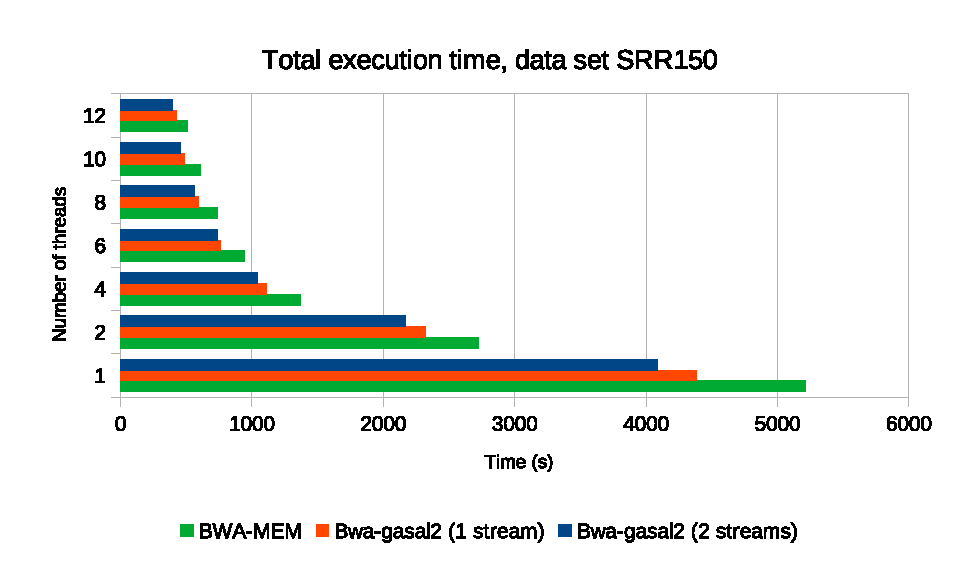
\includegraphics[width=1\textwidth]{srr150/total-exec-time-srr150}
		\caption{Total execution time for SSR150}
		\label{fig:total-exec-time-srr150}
	\end{subfigure}%
	
	\begin{subfigure}[b]{1\textwidth}
		\centering
		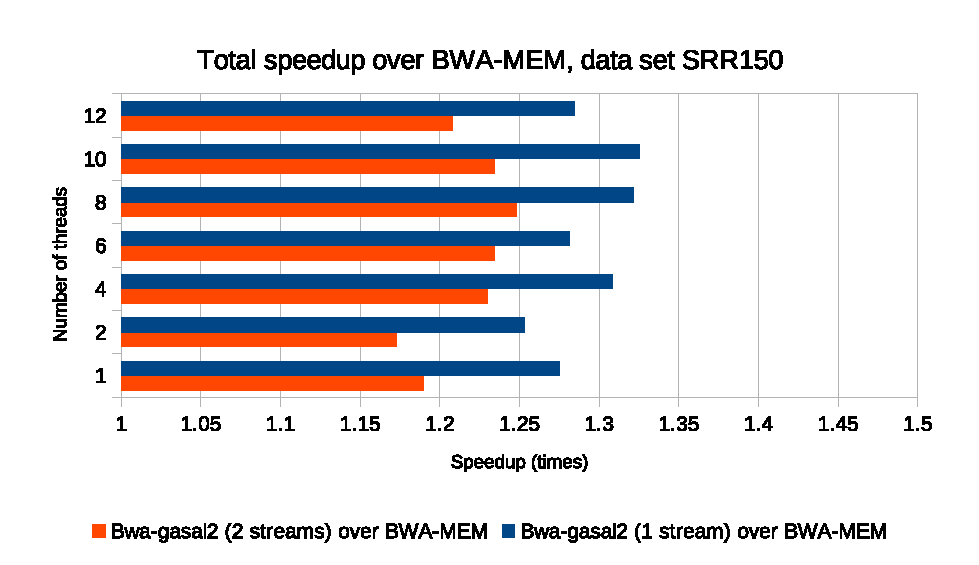
\includegraphics[width=1\textwidth]{srr150/total-exec-speed-up-srr150}
		\caption{Speed-up for the whole program execution for SRR150}
		\label{fig:total-exec-speed-up-srr150}
	\end{subfigure}
	\caption{Program results for data set SRR150}
	%\label{fig:}
\end{figure}


We obtain the most important speed-up using a single thread, reaching 1.35$\times$ the original program speed. This is promising, but is hardly a good indicator: in fact, these kind of program is usually run with multiple threads, and as we mentioned on chapter~\ref{chap:accel}, a single thread running the accelerator is far from sufficient to saturate the GPU computing resources.

In the case of 12 threads, we reach a GPU occupation of around 95\%, which is the kind of figure we are looking for. Here, the total speed-up almost reaches 1.28$\times$. It is substantially below our theoretical maximum of 1.37$\times$, but we are getting closer. Many factors can participate in making this difference. In particular, memory filling for the batches requires a significant amount of time on the CPU side, in addition to the memory copies from host to device. In this case, we started with an already large memory allocation, to avoid any overhead caused by new allocations.

In all cases, the difference between one and two streams is striking, with the speed-up even leaping from 1.21$\times$ to 1.28$\times$ in the 12 threads case.

When isolating the kernel times and kernel speed-up, we get the measurements shown respectively on figure~\ref{fig:kernel-exec-time-srr150} and figure~\ref{fig:kernel-exec-speed-up-srr150}. It is important to notice that what is reported as "kernel time" for the 2-stream variant represents the time during which the CPU is actively waiting for the GPU results. In other words, we have hidden-time execution disabled when using one stream, and enabled with 2 streams. We call this "visible kernel execution time".


\begin{figure}[p]
	\centering
	\begin{subfigure}[t]{1\textwidth}
		\centering
		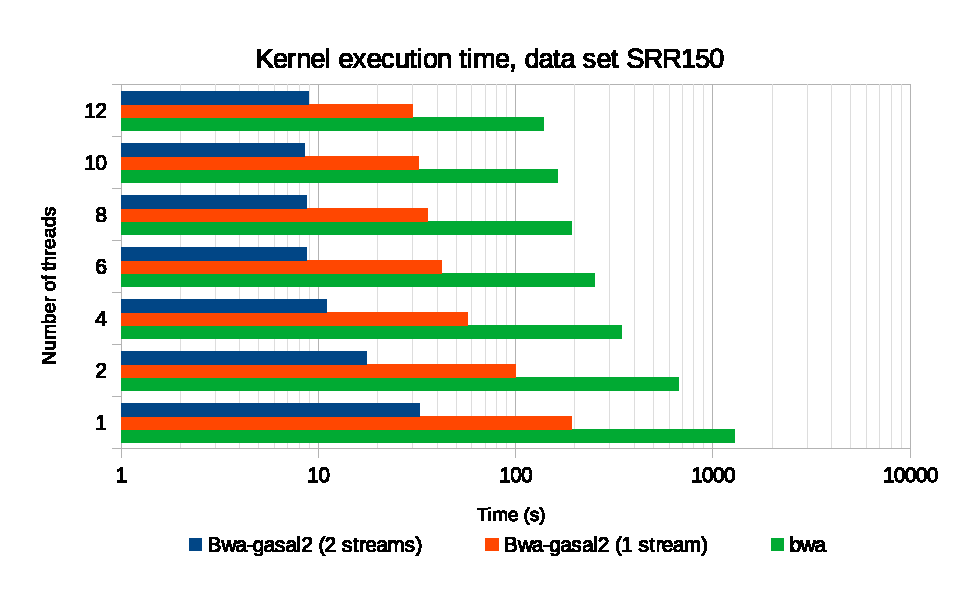
\includegraphics[width=1\textwidth]{srr150/kernel-exec-time-srr150}
		\caption{Visible kernel execution time for SRR150}
		\label{fig:kernel-exec-time-srr150}
	\end{subfigure}%
	
	\begin{subfigure}[b]{1\textwidth}
		\centering
		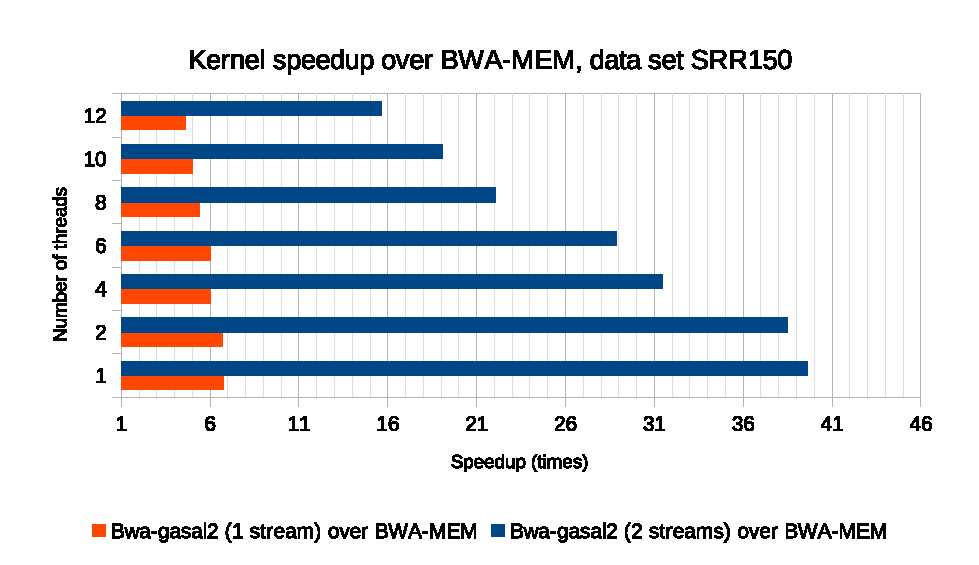
\includegraphics[width=1\textwidth]{srr150/kernel-exec-speed-up-srr150}
		\caption{Speed-up for the kernel execution for SRR150}
		\label{fig:kernel-exec-speed-up-srr150}
	\end{subfigure}
	\caption{Kernel results for data set SRR150}
	%\label{fig:}
\end{figure}

With hidden-time execution, on the 2-stream version, the visible kernel time is simply an order of magnitude shorter. In this special case, the kernel times were hugely different, so we had to display them in log scale. But while the visible sped-up reaches 4.7$\times$ on single streams with 12 threads, it jumps to almost 16$\times$, effectively shrinking down the visible compute time of the extension by the same amount. Although it is not useful in real-life, single-thread results are even more impressive, with a visible kernel speed-up reaching 40$\times$ with hidden-time, and only 6$\times$ when actively waiting for the result.


\subsection{Data set SRR250}

We run the same measurements on data set SRR250. Its sequences are longer, so they take quite a substantial amount of time to complete. Execution times and overall speed-up are shown on figure~\ref{fig:total-exec-time-srr250} and figure~\ref{fig:total-exec-speed-up-srr250} respectively.


\begin{figure}[p]
	\centering
	\begin{subfigure}[t]{1\textwidth}
		\centering
		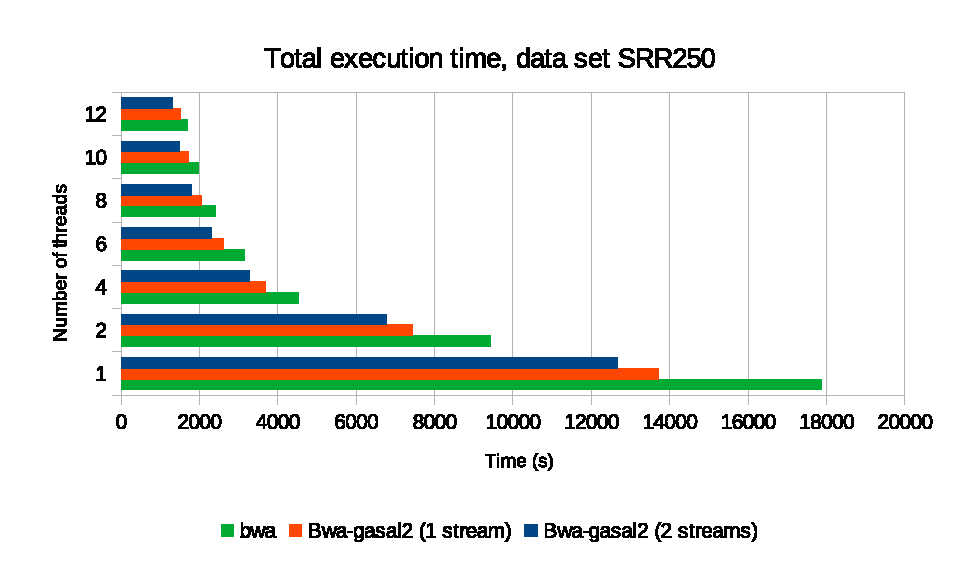
\includegraphics[width=1\textwidth]{srr250/total-exec-time-srr250}
		\caption{Total execution time for SSR250}
		\label{fig:total-exec-time-srr250}
	\end{subfigure}%
	
	\begin{subfigure}[b]{1\textwidth}
		\centering
		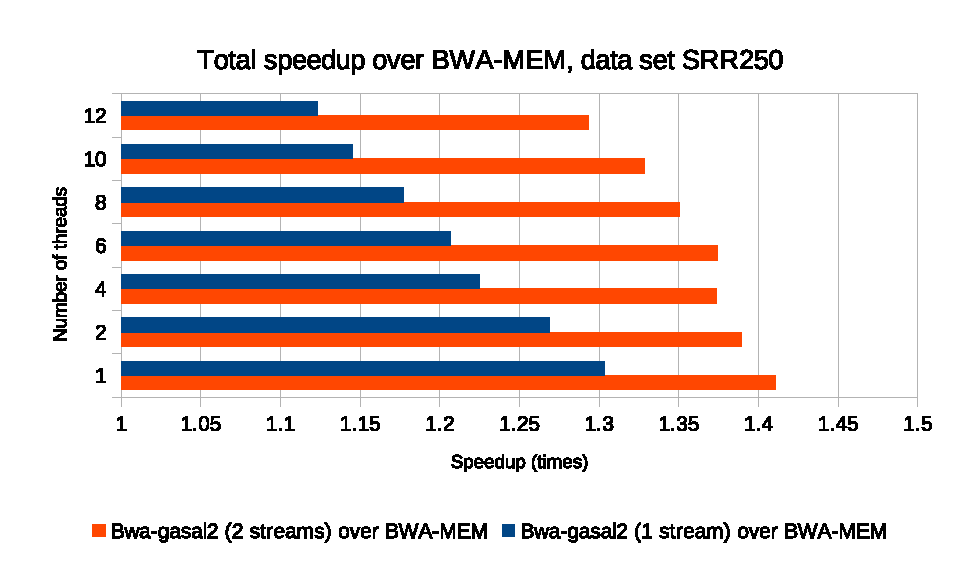
\includegraphics[width=1\textwidth]{srr250/total-exec-speed-up-srr250}
		\caption{Speed-up for the whole program execution for SRR250}
		\label{fig:total-exec-speed-up-srr250}
	\end{subfigure}
	\caption{Program results for data set SRR250}
	%\label{fig:}
\end{figure}

For this data set, the extension time is taking approximately 33\% of the total time, so we would expect a bigger speed-up, with the theoretical maximum being 1.5$\times$. However, it is not what we observe, even in the best case with 2 streams: on a single thread, we can effectively reach a speed-up of 1.41$\times$, which gets somewhat close to the theoretical maximum, but with 12 threads, we reach only 1.29$\times$. This is still a valuable improvement over the original version, and in all cases, hidden-time execution gives a substantial boost in performance. When comparing the single stream version to its 2-stream counterpart, we note that using 2 streams definitely helps shrinking the execution time.

Let's examine the kernel times and speed-up, on figure~\ref{fig:kernel-exec-time-srr250} and~\ref{fig:kernel-exec-speed-up-srr250} respectively.


\begin{figure}[p]
	\centering
	\begin{subfigure}[t]{1\textwidth}
		\centering
		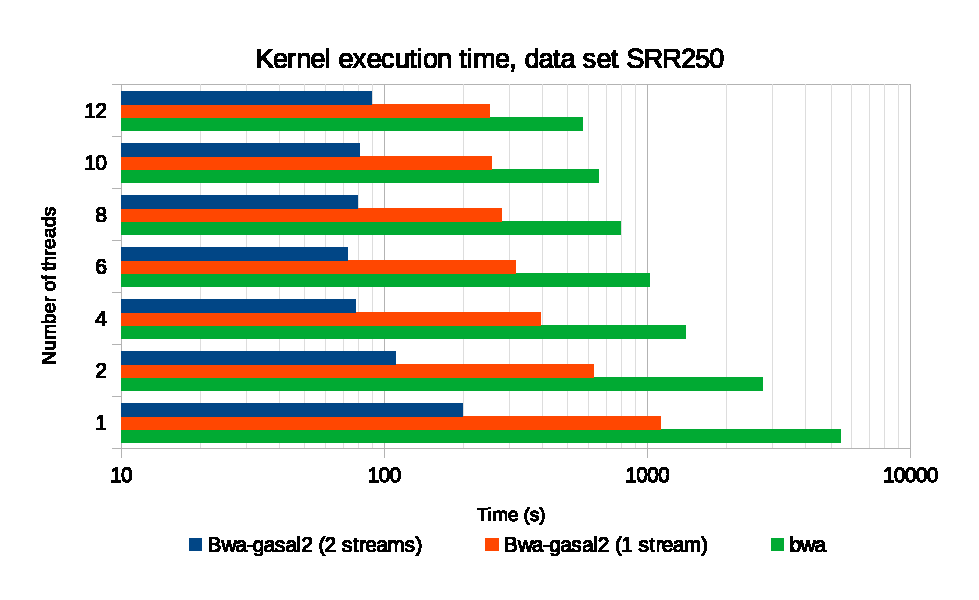
\includegraphics[width=1\textwidth]{srr250/kernel-exec-time-srr250}
		\caption{Visible kernel execution time for SRR250}
		\label{fig:kernel-exec-time-srr250}
	\end{subfigure}%
	
	\begin{subfigure}[b]{1\textwidth}
		\centering
		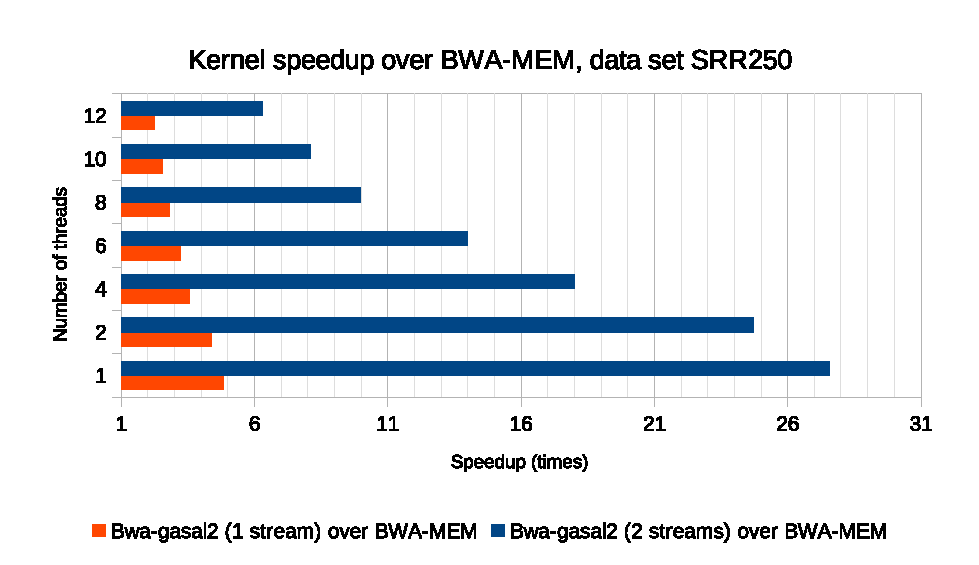
\includegraphics[width=1\textwidth]{srr250/kernel-exec-speed-up-srr250}
		\caption{Speed-up for the kernel execution for SRR250}
		\label{fig:kernel-exec-speed-up-srr250}
	\end{subfigure}
	\caption{Visible kernel execution for data set SRR250}
	%\label{fig:}
\end{figure}

Kernel running times for BWA (running on CPU) are somewhat steady. As the number of threads increases, we get closer to a plateau as the execution time hardly gets any lower for all programs. Again, we can remark how hidden-time execution helps in computing it faster with two streams. The difference is tremendously high for one thread, with time the CPU waiting for the GPU to complete being 5 times lower with 2 streams (from 1125s with 1 stream to 197s), but the benefits are not as high when using 12 threads, with the kernel waiting time being only 2.5 lower for the 2-stream version (from 250s for 1 stream to 89s for 2 streams). When using multiple threads, the overhead caused by filling a lot of GPU batches then copying them to the device is more important. It is all the more the case when using twice as many streams, having twice as many structures needing filling and being copied to the device.

We can also see whether increasing the number of streams could give any performance improvement. Results are shown on figure~\ref{fig:exec-time-nbstreams}. As we can see, more than 2 streams does not result in any improvement. 

\begin{figure}[h]
	\centering
	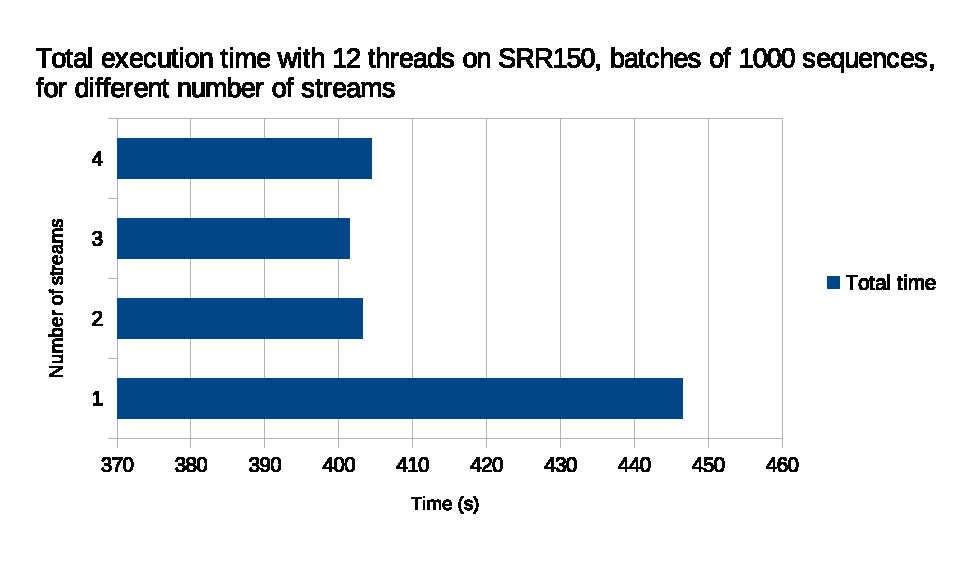
\includegraphics[width=0.9\linewidth]{exec-time-nbstreams}
	\caption{Execution time for 12 threads and different number of streams, data set SRR150}
	\label{fig:exec-time-nbstreams}
\end{figure}

% Note: this newpage is nice here, but depending on the content above, it may be ugly.
% \newpage
		
		\section{Correctness measurement}
		
As explained before, we use the \verb|diff| utility to compare two SAM output files. Having the number of different lines between two files, we can calculate a percentage of difference. To be able to compare the outputs, they must be in the same order: this is why we have to run the program on single thread for this verification. We measure the influence of the seed-only paradigm on the results. It is worth noting that, in addition to the best alignment with its score, BWA outputs alternative alignments which may lead to different, lower quality results. In the case of seed-only paradigm, it regularly happens that the main result is matching, yet the secondary alignments present very slight differences. Since these values are rarely useful in real use cases, we also compared the outputs without these results, to know the difference only for the final alignment. We implemented a "seed-only" version of BWA to control that our kernel implementation on GPU is correct. The results are presented on Figure~\ref{fig:result-diff-srr150}.

\begin{figure}[h!]
	\centering
	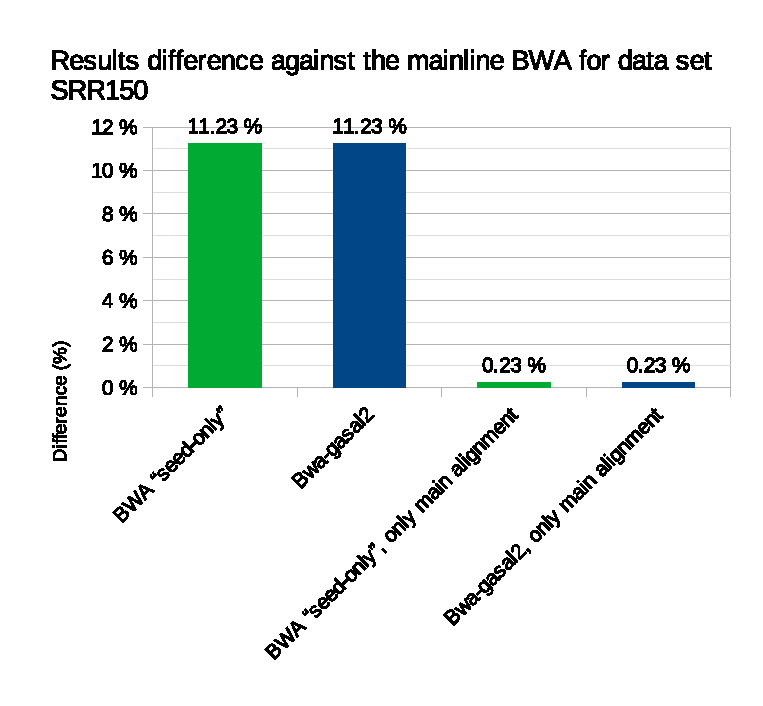
\includegraphics[width=1\linewidth]{srr150/result-diff-srr150}
	\caption{Difference in the result with the mainline version of BWA}
	\label{fig:result-diff-srr150}
\end{figure}

First, we checked that the results between the seed-only version of BWA and our bwa-gasal2 have the same output. They present the same number of difference with the mainline program, and have the same content.

We notice that the seed-only paradigm globally introduces a noticeable number of differences. 11.23\% of the lines are not matching. Still, when we set aside the secondary results, this percentage drops to a mere 0.23\%. This is small enough to consider it acceptable.



		
		\section{Memory use measurement}
		GPU memory use grows strictly linearly with respect to the number of streams and threads. When going from one to two streams, bwa-gasal2 takes twice as much memory. In this section, we will present the case we deemed more representative of real use.

GPU memory (VRAM) use is a delicate topic to assess, since it highly depends on various factors:

\begin{itemize}
	\item the GPU, since the VRAM available may not be sufficient to saturate its computing resources,
	\item the CPU, because how many threads we can instantiate directly impacts how much VRAM we will need,
	\item the RAM, since the sequences also need to be loaded in RAM before being copied to the GPU (although this is rarely a limiting factor, since a given machine has far more RAM than its GPU has VRAM),
	\item and of course, the data set running.
\end{itemize}

We cannot conduct measurements that are corresponding to any algorithmic truth in this case. Consequently we will present the memory use as a case study corresponding to our current machine and data sets, and we will see if, in our example case, the memory use can be deemed as reasonable. We consider the GPU we used (Tesla K40c) with its 2880 CUDA cores and its 12GB or VRAM, as representative of the accelerators generally used.

For this, we start bwa-gasal2 with a substantial low amount of memory, and let the automatic memory extension grow until the end of the program. The memory use for data set SRR150 and SRR250 is shown on figure \ref{fig:memory-use}. We measured memory use for what we consider a regular use case for our machine : 12 threads, with 2 streams. 

\begin{figure}[h]
	\centering
	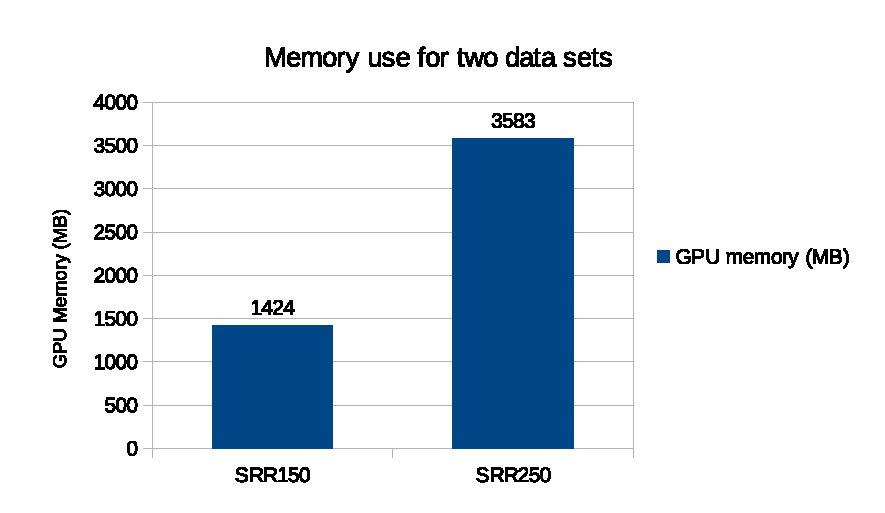
\includegraphics[width=0.9\linewidth]{memory-use}
	\caption{Memory use for our two data sets on our testing machine}
	\label{fig:memory-use}
\end{figure}

On these examples, we need around 1570 MB for a data set with sequences of 150 bases, and 2730 MB for sequences 250 bases long. This shows that our solution will not properly scale with very long sequences, since we will quickly run out of memory for our GPU. Still it is decent for our short-length sequences, where we use less than 1/6th of our total available memory with our worst case scenario. In particular, this allows to use a cheaper accelerator if needed, and in our case, it leaves more memory to accelerate in the future another part of the calculation.

	
	\chapter{Conclusions and recommendations}
	\label{chap:ccl}
	In this chapter, we present the main conclusions of the thesis and reflect back on the research questions defined in the thesis. We also discuss a number of recommendations for future work. %Let's recapitulate the progress made by this work.
	
		\section{Conclusion}
		

In this thesis, we addressed the challenge of accelerating time consuming genomics algorithms to make them more accessible for application in the field. The thesis specifically focuses on BWA-MEM as one of the most widely used DNA read mapping programs. 

Below are the research questions we defined in the thesis, and the answers we can provide.

\begin{itemize}
	\item How can we accelerate DNA alignment in an already existing program?
\end{itemize}	

We chose an industry standard mapper, BWA-MEM, and we accelerated one of its processing stages. The "seed-extension" phase can be run in a accelerated on a dedicated hardware, the GPU. We integrated the library GASAL2 in BWA-MEM to realise the acceleration. Still, we could not directly compute seed-extension as done in original BWA-MEM. In BWA-MEM, the left and right parts were computed one after the other, and starting with the previous total score (so, first the seed score is used to compute the left part, then the score from the left alignment is used for the right part). Instead, we compute both parts at the same time only using the seed score as starting score.

To produce a working piece of software, we had to implement multiple improvements in GASAL2. We created a dedicated kernel for extension, copying BWA-MEM behaviour that follows the Smith-Waterman algorithm, but able to start with any given starting score. We also needed to implement an extensible memory structure for GASAL2 to adapt to an unknown number of alignment with unpredictable lengths for each of them. Finally, we instrumented both the new version bwa-gasal2 and BWA-MEM to be able to log their execution time and compare them. 

We started from the demonstrator GASE-GASAL2 (based on BWA-MEM) that we ported to support C++ compilation before integrating the new GASAL2 version. It features templates for generic functions and a parameters class. We implemented all the aforementioned features to produce the current version of the software, \textbf{bwa-gasal2}.

\begin{itemize}
	\item How much speed-up can we get from GPU acceleration?
\end{itemize}

We ran our solution on two data sets, with reads of 150 and 250 bases, named SRR150 and SRR250 respectively. Depending on the data, inn BWA-MEM, extension takes between 27\% and 33\% of the total time. This means that, depending on the situation, we can reach a theoretical 1.37$\times$ and 1.50$\times$ speed-up.

We saw that on our test machine, parallel execution alone can provide an already interesting speed-up. On 12 threads in SRR150, we reach 1.21$\times$ speed-up. But when enabling overlap execution with two CUDA streams, we can get a 1.28$\times$ speed-up, which gets closer to the theoretical maximum of 1.37$\times$. This is all the more visible with data set SRR250 where the speed-up soars from 1.12$\times$ to 1.28$\times$. We obtained a very good acceleration, close to the theoretical maximum. 

There are various reasons explaining the difference between achieved and maximum speedup. First, the CPU has to wait to get the final result of a given pack of sequences (it cannot start the next pack right away). Moreover, some overhead is introduced when filling the data structure in GASAL2 on the host side, before copying them on the device.

\begin{itemize}
	\item How close can the results with a different computing method be to the original software?
\end{itemize}

Since the output is text-based, we compared them by logging them to text and using the \verb|diff| UNIX utility. For each sequence, the main alignment is reported, along with secondary scores that are not always listed in the same order, and can slightly differ because of the ``seed-only" paradigm.

When comparing the complete results from the SRR150 data set, we found a 11.23\% difference. This is a higher bound that includes non similar secondary score order. This information is usually not important in downstream analysis. This is why we also compared only using the main alignment, and also discarding the low quality scores (lower than 20). In this last case, the difference drops to 1.82\%, so the two outputs are very similar. We concluded that our solution produces acceptable results.

\begin{itemize}
	\item How to ensure that the GPU resources are well used, while leaving more space if needed for future evolution?
\end{itemize}

A GPU is well used when its computing resources have a high utilisation. Although a single kernel execution from GASAL2 has a low utilisation (between 8\% to 15\%), instantiating multiple CPU threads to launch more kernels at the same time allows us to multiply this utilisation in a direct fashion. This way, we can reach 70\% with peaks at 90\% of utilisation, which is a good use of resources.

On the contrary, a sane use of GPU VRAM would be not to use more memory than what is necessary. Being frugal in memory can be useful if we want to align longer sequences, as these take a lot of space. Also, it can prevent out-of-memory errors if other parts were accelerated, or simply it could allow the program to run on a moderately-sized accelerator. To this extent, we used extensible memory structures to store the DNA strings, with a linked list structure with elements growing in size. This allows to allocate more memory whenever needed, and since the linked list is re-used, we try to keep the number of memory allocations to the minimum. With this, we could use around 20\% of the total memory of our accelerator for data set SRR150, or around 30\% for SRR250. 


		
		\section{Future work}		
		Concerning what lies ahead, the first notice is about bwa-gasal2 licencing. Originally, BWA is under GNU General Public License v3.0 and GASAL2 is licenced under Apache 2.0 License. Because of the licence choice of BWA, projects including it must follow the GPL v3.0, providing full source code disclosure. It follows that bwa-gasal2 will get the same licence to respect BWA original rights; this includes leaving the source open for anyone to see. This means that any volunteer can contribute or fork the project to enlarge it, provided they ship it with the same licence.

The first feature that would be highly valuable in bwa-gasal2 is seeding acceleration. As we have seen, seeding is the more lengthy step, taking approximately half of the time for short sequences. It is crucial to implement acceleration for it to gain major speed-up for the program as a whole. 

Other optimisation can be designed, in particular to the extension kernel. Any optimisation done at this level could have serious repercussions on the total execution time. For example, one could implement data packing on a 3-bit encoding, to save more memory and compute the dynamic programming matrix by tiles of $10 \times 10$ bases. It would be interesting whether this could bring a noticeable speed-up.

		\section{Closing and thanks}
		\input{503-closing}
	
	\printbibliography

\end{document}